%Przykładowy plik ułatwiający złożenie projektu dyplomowego inżynierskiego.
%UWAGA: Generowany napis na stronie tytułowej o treści PROJEKT DYPLOMOWY INŻYNIERSKI został zaproponowany przeze mnie i nie jest, póki co, potwierdzony przez władze wydziału. Przed ostatecznym oddaniem tak złożonej pracy należy upewnić się jaka powinna być treść tego napisu. W momencie gdy uzyskam informację na temat treści tego napisu, dokonam niezbędnych zmian w źródłach.

\documentclass[eng,printmode]{mgr}
%opcje klasy dokumentu mgr.cls zostały opisane w dołączonej instrukcji

%poniżej deklaracje użycia pakietów, usunąć to co jest niepotrzebne
\usepackage{polski} %przydatne podczas składania dokumentów w j. polskim
%\usepackage[polish]{babel}%alternatywnie do pakietu polski, wybrać jeden z nich
\usepackage[utf8]{inputenc} %kodowanie znakĂłw, zaleĹĽne od systemu
\usepackage[T1]{fontenc} %poprawne składanie polskich czcionek

%pakiety do grafiki
\usepackage{graphicx}
%\usepackage{subfigure}
\usepackage{psfrag}

%pakiety dodające dużo dodatkowych poleceń matematycznych
\usepackage{amsmath}
\usepackage{amsfonts}

%pakiety wspomagające i poprawiające składanie tabel
%\usepackage{supertabular}
\usepackage{array}
\usepackage{tabularx}
\usepackage{hhline}

\usepackage{mathtools}
\usepackage{listings}


%pakiet wypisujący na marginesie etykiety równań i rysunków zdefiniowanych przez \label{}, chcąc wygenerować finalną wersję dokumentu wystarczy usunąć poniższą linię
%\usepackage{showlabels}

%definicje własnych poleceń
\newcommand{\R}{I\!\!R} %symbol liczb rzeczywistych, działa tylko w trybie matematycznym
\newtheorem{theorem}{Twierdzenie}[section] %nowe otoczenie do składania twierdzeń

%dane do złożenia strony tytułowej
\title{Detekcja aktywności mówcy w systemach automatycznego rozpoznawania mowy}
\engtitle{Voice activity detection in automatic speech recognition systems}
\author{Paulina Szczerbak}
\supervisor{Prof. dr hab. inż. Ryszard Makowski}
%\guardian{dr hab. inż. Imię Nazwisko Prof. PWr, I-6} %nie używać jeśli opiekun jest tą samą osobą co prowadzący pracę

%\date{2008} %standardowo u dołu strony tytułowej umieszczany jest bieżący rok, to polecenie pozwala wstawić dowolny rok

%poniżej jest lista kierunków i specjalności na wydziale elektroniki, należy wybrać właściwe lub dopisać jeśli nie ma odpowiednich
\field{Automatyka i Robotyka}
\specialisation{Technologie informacyjne w systemach automatyki (ART)}

%tutaj zaczyna się właściwa treść dokumentu
\begin{document}
\bibliographystyle{plabbrv} %tylko gdy uĹĽywamy BibTeXa, ustawia polski styl bibliografii

\maketitle %polecenie generujące stronę tytułową
%\dedication{6cm}{Dla mamy i taty heheheheheh xD \texttt{$\backslash$dedykacja}}

\tableofcontents %spis treści

%poniżej znajduje się przykładowa treść dalszej części dokumentu, zainteresowanych zachęcam do rozszyfrowania frazy "Lorem ipsum" :)
\chapter{Wstęp}
Celem niniejszej pracy jest zaprezentowanie wybranych metod detekcji aktywności mówcy (VAD) w systemach automatycznego rozpoznawania mowy w oparciu o napisany program w języku C++. Kolejnym etapem jest porównanie zaimplementowanych metod pod względem dokładności detekcji w separowanych wyrazach oraz w dłuższych ciągach słów.\vspace{3mm}

Rozdział 2. opisuje w uproszczony sposób proces wytwarzania mowy przez człowieka. Prezentuje, w jaki sposób działa aparat mowy oraz z jakich narządów się składa. Na koniec pokazany jest matematyczny model jaki można stworzyć wzorując się na naturalnym systemie generowania mowy.\vspace{3mm}

Rozdział 3. zawiera wyjaśnienie na temat detekcji aktywności mówcy - czym jest oraz gdzie jest wykorzystywana. W tym rodziale opisane są również wybrane algorytmy, które zostały zestawione w dalszej części pracy. Przedstawiona jest zasada ich działania oraz pokrótce wyjaśniona kwestia implementacyjna każdego z nich.\vspace{3mm}
 
Rozdział 4. objaśnia niektóre aspekty implementacyjne programu.\vspace{3mm}

Rozdział 5. przedstawia sposób oceny wyników. Zawiera  wyniki detekcji dla pojedynczych słów oraz całych ciągów. Na końcu tego rozdziału znajduje się również ostateczne porównanie w działaniu wybranych algorytmów i ich ocena.\vspace{3mm}

\chapter{Generowanie sygnału mowy}
 \section{Mowa w życiu człowieka}
 
 Mowa w życiu większości ludzi stanowi podstawę komunikacji interpersonalnej. Jest sygnałem akustycznym, czyli rozważany jest zakres częstotliwości słyszanych przez człowieka, to jest od 20Hz do 16kHz. Zatem mowa to nic innego jak system artykułowanych dźwięków, które układają się zgodnie z konwencją wybranego języka. Pełni ona funkcję nie tylko komunikacyjną (przekazywanie informacji drugiej osobie o tym, co doświadczyliśmy, czy czego się dowiedzieliśmy), ale również ekspresyjną (można w niej zawrzeć informacje o emocjach nadawcy) oraz regulacyjną (wydawanie i przyjmowanie dyspozycji). 
 
 
 \section{Biologiczny proces generowania mowy}
 Wszelkie metody przetwarzania sygnału mowy muszą bazować na strukturze sygnału, a ta jest niewątpliwie uzależniona od sposobu, w jaki jest on wytwarzany. Niegdyś generowanie sygnałów mowy było domeną jedynie organizmu człowieka, czyli systemu naturalnego. W celu stworzenia systemu, który w jakiś sposób operuje na sygnałach mowy, czyli np. syntezatora mowy, systemu generującego sygnały mowopodobne, systemu automatycznego rozpoznawania mowy czy detekcji aktywności mówcy, należy mieć przynajmniej podstawową wiedzę na temat systemu naturalnego - tego, w jaki sposób działa aparat mowy człowieka.
 
 Wytwarzanie mowy przez człowieka jest procesem niezwykle skomplikowanym, który ma swój początek w mózgu, gdzie następuje konstrukcja wypowiedzi. Później następuje sformułowanie fonetyki i artykulacja poprzez aparat mowy. Ponadto, w procesie generowania mowy można wyróżnić cztery pomniejsze etapy:
	 
	 - proces psychologiczny - wymyślenie i skonstruowanie wypowiedzi,
	 
	 - proces neurologiczny - pobudzenie przez układ nerwowy mięśni, które biorą udział w wytwarzaniu mowy,
	 
	 - proces fizjologiczny - proces kształtowania dźwięków mowy ludzkiej,
	 
	 - proces aerodynamiczny - drgania i przepływ powietrza przez aparat mowy. 
  
  Pierwszym narządem wchodzącym w skład traktu głosowego człowieka są płuca - dostarczają one powietrze do procesu artykulacji, są źródłem zmian ciśnienia akustycznego. Organ mowy człowieka jest napędzany przez wydychane powietrze. Powietrze to, jest prowadzone przez oskrzela i tchawicę do krtani, a drgające w niej struny głosowe modyfikują ciśnienie i wytwarzają dźwięczne fragmenty mowy.  Następnie, dzięki wnękom rezonansowym, tworzonym przez język, podniebienie, zęby oraz wargi, dźwięk ten jest modulowany. 

\begin{figure}
	Niezwykle ważną rolę przy formowaniu tych wnęk, odgrywają ruchy żuchwy i policzków. Podczas generowania głosek nosowych zamknięta jama ustna spełnia rolę bocznika akustycznego, a dzięki odpowiedniemu ustawieniu języczka podniebienia miękkiego, fala dźwiękowa jest emitowana przez jamę nosową i nozdrza. Struktura traktu głosowego jest przedstawiona schematycznie na rysunku 2.1.
	\begin{center}
		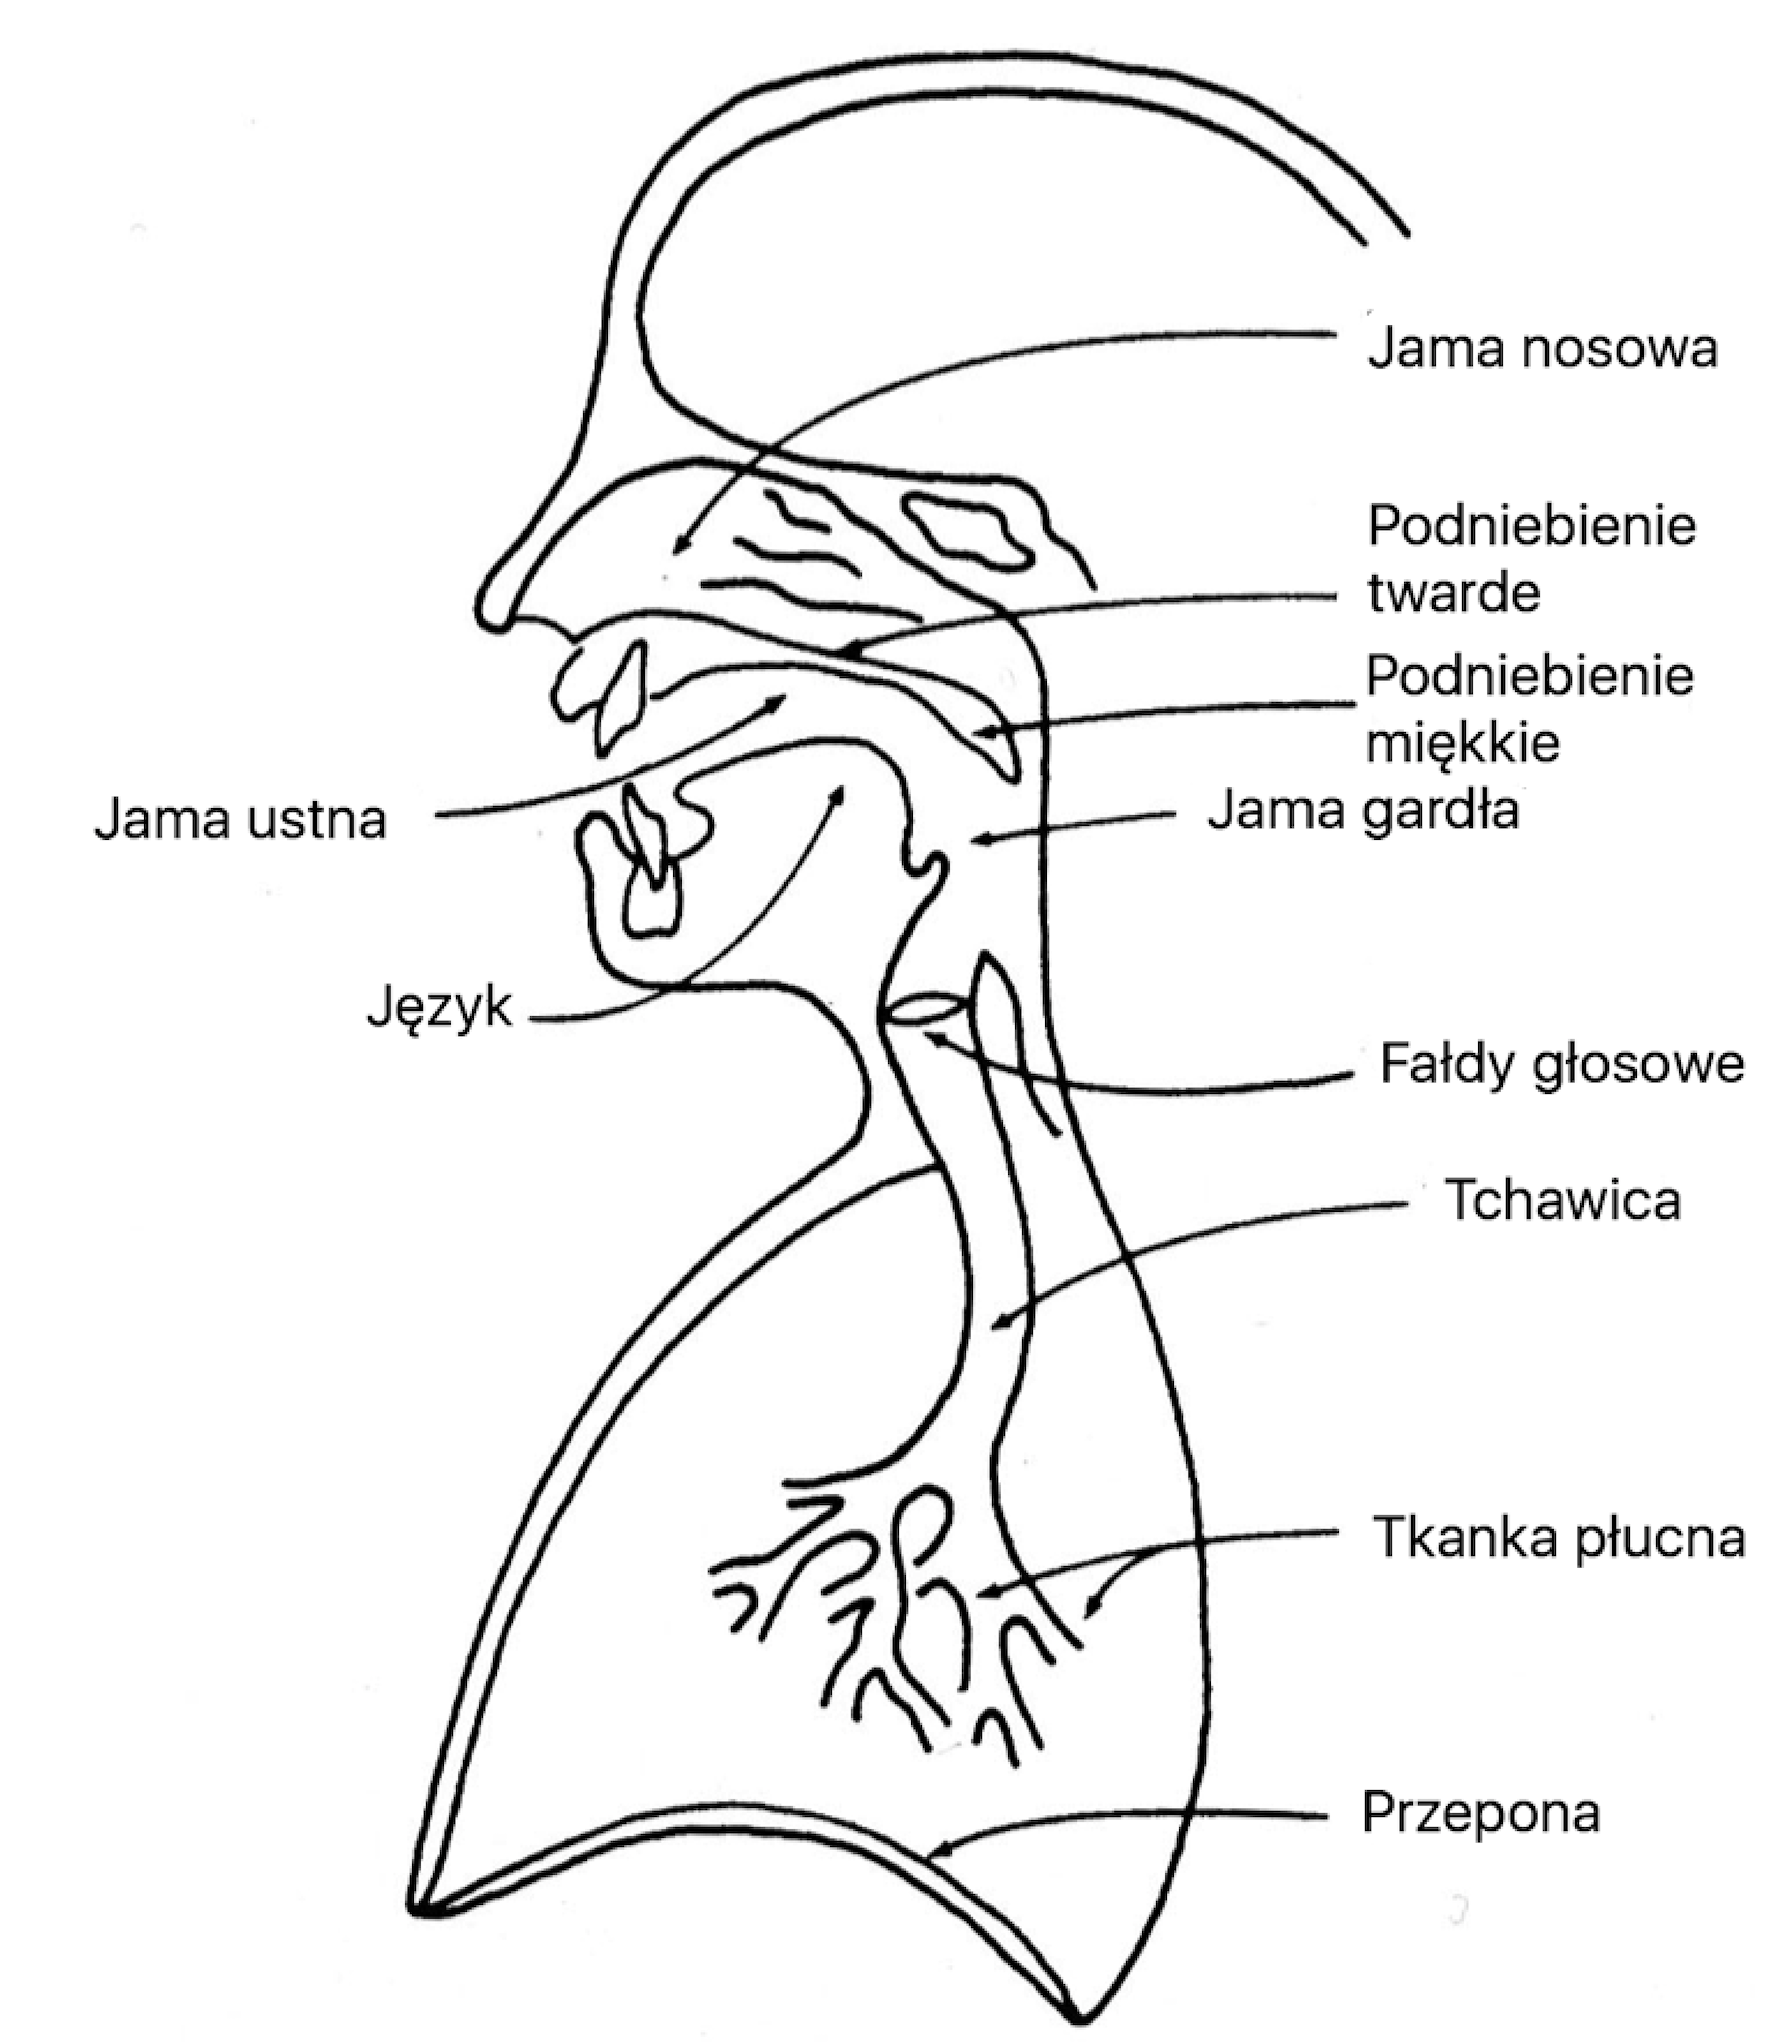
\includegraphics[scale=0.25]{speechmechpl.png}
		\caption{Aparat mowy człowieka}\vspace{5mm}
	\end{center}

	 Ponadto, sterowanie całym systemem generowania mowy jest bardzo złożone i w dużej mierze opiera się na licznych sprzężeniach zwrotnych. Główną rolę odgrywa tutaj sprzężenie zwrotne, które poddaje jakość wydawanych dźwięków bezpośredniej ocenie poprzez analizator słuchowy. Dzięki temu proces artykulacji jest odpowiednio sterowany. Istotę tego sprzężenia zwrotnego potwierdzają trudności z mową wśród ludzi głuchych oraz ludzi słyszących, którzy tymczasowo przebywają w trudnych warunkach środowiskowych, które uniemożliwiają słyszenie własnego głosu.\vspace{5mm}
 
	 \begin{center}
	 	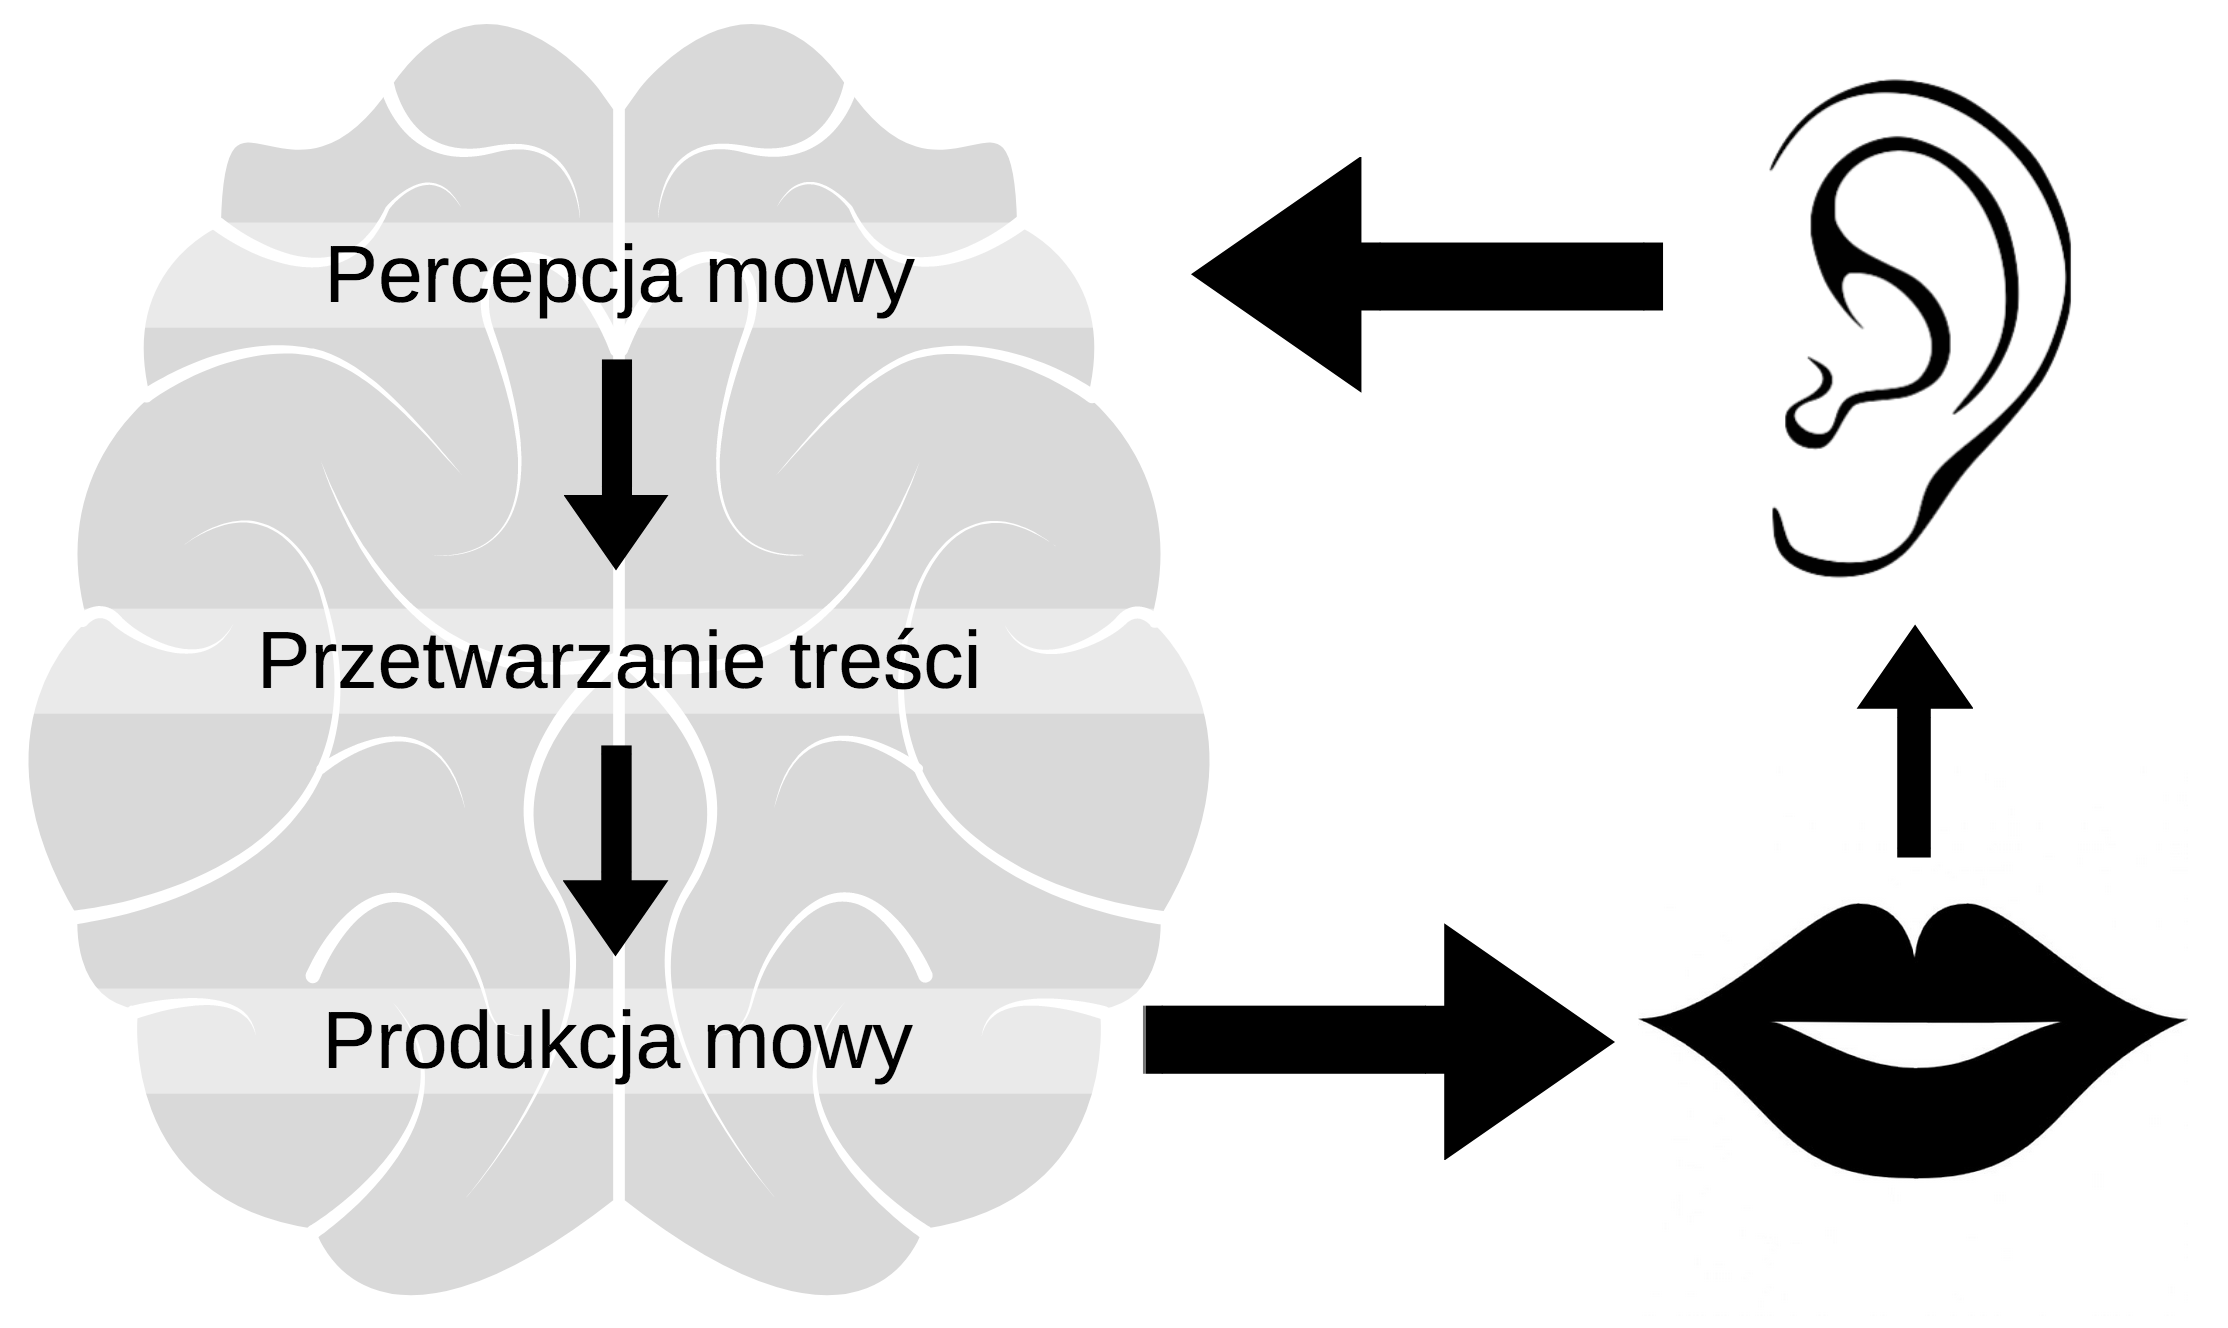
\includegraphics[scale=0.25]{feedback.png}
	 	\caption{Sprzężenie zwrotne w wytwarzaniu mowy} 	
	 \end{center}
 \end{figure}
 
\begin{figure}
 	\section{Sygnał w dziedzinie czasu oraz w dziedzinie częstotliwości}
 	\begin{center}
 		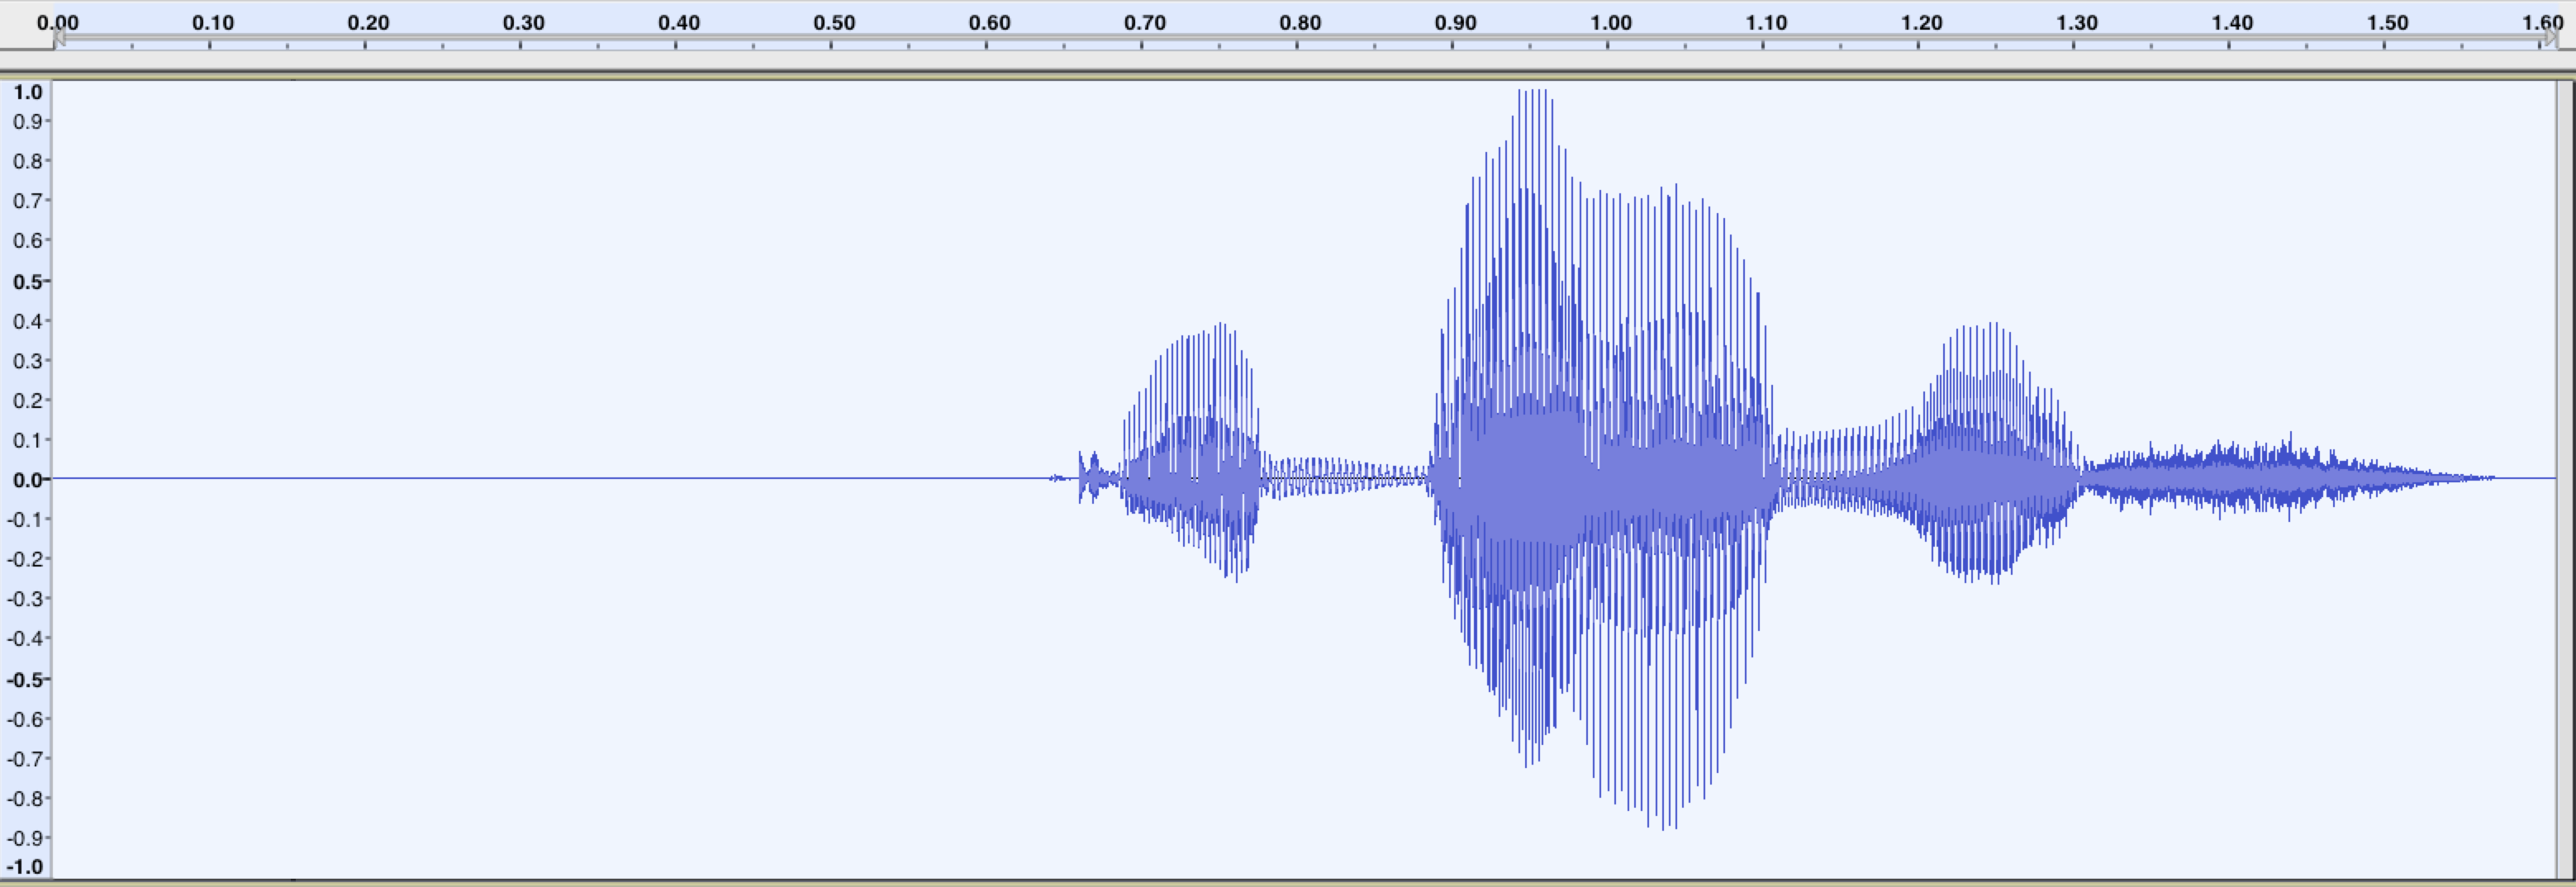
\includegraphics[scale=0.3]{kabanosTime.png}
 		\caption{Przebieg sygnału w dziedzinie czasu dla słowa \emph{kabanos}}\vspace{5mm}
 		
 		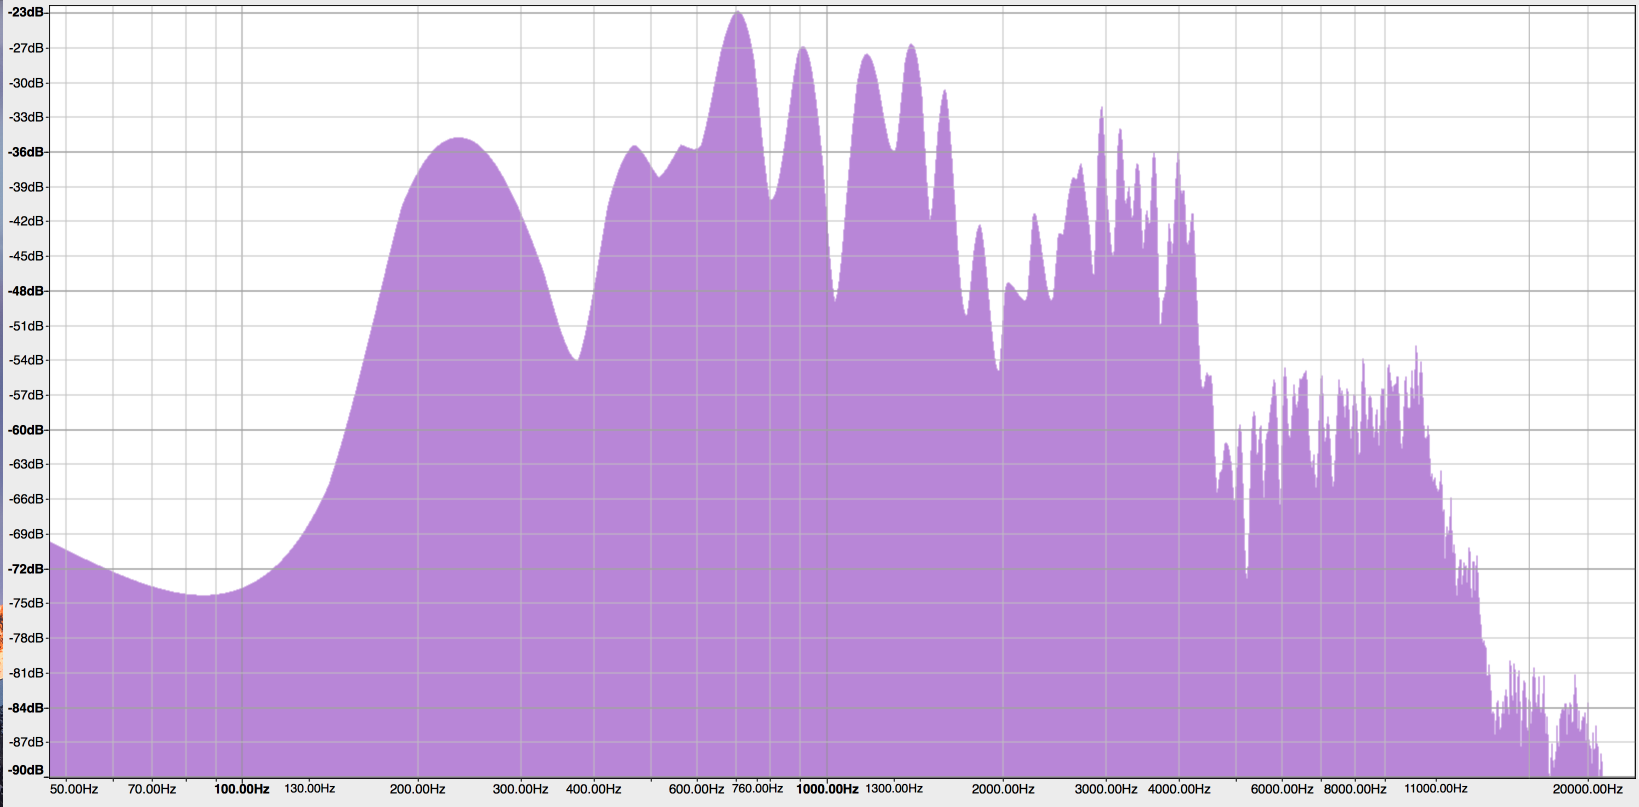
\includegraphics[scale=0.5]{kabanosSpectrum.png}
 		\caption{Widmo sygnału dla słowa \emph{kabanos}}\vspace{5mm}
 	\end{center}
\end{figure}
  
 
\chapter{Wybrane metody detekcji aktywności mówcy}
 \section{Czym jest detekcja aktywności mówcy oraz gdzie się ją wykorzystuje}
 
 Detekcja aktywności mówcy (Voice Activity Detection - VAD) jest powszechnie stosowana w systemach automatycznego rozpoznawania mowy. Podczas rejestrowania wypowiedzi do późniejszego przetwarzania jej przez system ARM, zostaje zarejestrowana cała wypowiedź mówcy, włącznie z częścią, która nie zawiera mowy. Jeżeli we fragmencie jest zawarty sygnał mowy, mówimy, że mówca jest aktywny. Aktywnością mówcy nazywa się emitowny przez niego dźwięk.  Zawartość semantyczna wypowiedzi jest zawarta w głównej mierze we fragmentach, kiedy mówca jest aktywny. Analizowanie całego  zarejestrowanego sygnału mowy, bez wykorzystania systemu VAD, jest oczywiście możliwe, aczkolwiek niepotrzebnie zwiększa czas obliczeń oraz istnieje prawdopodobieństwo, że fragment, gdy mówca nie jest aktywny, zostanie błędnie zaklasyfikowany jako jakiś konkretny fonem - zatem w dużej mierze może popsuć jakość rozpoznania. Detekcja aktywności mówcy w ogólnym przypadku zakłada, że sygnał może występować w dwóch stanach: tylko szum (brak sygnału mowy), szum + sygnał mowy. Korzystając z zagadnienia hipotez ze statystyki, możemy pierwszy stan oznaczyć jako hipotezę $H_{0}$, a drugi jako $H_{1}$, dzięki czemu możemy przedstawić to w następujący sposób:
 \begin{equation}
  \begin{array}{c}
	  H_{0}: f(n)=x(n)\\
	  H_{1}: f(n)=v(n)+x(n)
  \end{array} 	 
 \end{equation}
  Przy takim rozumowaniu konieczne jest określenie statystyki $S(n)$ sygnału, dzięki czemu możliwe będzie dokonywanie detekcji, a w dalszej kolejności zastosowanie kryterium decyzyjnego. Kryterium decyzyjne zwykle polega na porównaniu wartości $S(n)$ z progiem detekcji, który w mniej skomplikowanych algorytmach przyjmuje stałą wartość. Natomiast w tych bardziej złożonych, może występować np. jako funkcja czasu. Wartość stałej wartości progu jest ustalana w wyniku teoretycznych rozważań lub empirycznie. Zatem detekcja $\gamma(n)$, w ogólnej postaci, będzie prezentować się następująco:
   \begin{equation}
   \begin{array}{c}
	   S(n)\geq\gamma(n)\to H_{1}\\
	   S(n)<\gamma(n)\to H_{0}
   \end{array} 	 
   \end{equation}
 
	 
 \section{Metoda bazująca na energii sygnału z adaptacyjnym współczynnikiem skalującym}
 
 Najbardziej powszechną metodą do obliczenia energii dla całego pasma  w sygnale mowy jest:
 
 $$ E_{j} =\frac{1}{N}\sum_{i=(j-1)N+1}^{jN}x^2(i)$$
 
 \hspace{8cm}gdzie: $E_{j}$ - energia j-tej ramki
 
 
  \subsection{Początkowy próg detekcji}
  Początkowa wartość progu jest ważna dla jego dalszego rozwoju - ponieważ będzie się zmieniał zgodnie ze śledzonym poziomem szumu w sygnale. Przyjęto, że początkowe 100 ms nagrania nie zawiera mowy. Jest to podyktowane tym, że mówca potrzebuje czasu na rekację, nabranie powietrza, aktywację strun głosowych. Te 100 ms są uznawane za przebieg pozbawiony sygnału mowy i ich średnia wartość obliczana jest zgodnie z powyższym wzorem.
  
  \subsection{Próg detekcji zmieniający się dynamicznie w czasie}
  Główną ideą tego algorytmu jest możliwośc obilczenia progu detekcji bez potrzeby korzystania z obszarów niezawierajacych mowy. Wykorzystywana jest minimalna oraz maksymalna energia sygnału mowy.   
  
  Innym popularnym sposobem na obliczenie energii sygnału mowy jest pierwiastek ze średniokwadratowej wartości energii (root mean square energy - RMSE), dany jako:
  
  $$ E_{j} =\sqrt{\frac{1}{N}\sum_{i=(j-1)N+1}^{jN}x^2(i)}$$
  
  'Dynamiczny' VAD jest oparty o obserwację, że estymata mocy sygnału mowy pokazuje wyraźne szczyty i doliny. Podczas gdy szczyty odpowiadają aktywności mowy, doliny mogą zostać wykorzystane do uzyskania estymaty mocy szumu. Ponadto, RMSE jest bardziej odpowiedni.
  
  \subsection{Wyznaczanie progu}
 Estymacja progu bazuje na poziomach energii $E_{min}$ oraz $E_{max}$ otrzymane z ciągu nadchodzących ramek. Te wartości są trzymane w pamięci i próg $\theta$ jest obliczany jako:
 
 $$\theta = k_{1}E_{max} + k_{2}E_{min}$$
 
  \hspace{8cm} gdzie $k_{1}$ i $k_{2}$ to współczynniki 
  
  \hspace{8cm}wykorzystane do interpolacji wartości
  
  \hspace{8cm} progu dla optymalnych wyników.\vspace{5mm} 
  
  Jeżeli energia bieżęcej ramki jest mniejsza niż wartość progu, ramka zostaje oznaczana jako niezawierająca mowy. 
  
  Jako, że mogą się pojawić pewne anomalie spowodowane zbyt niską energią, wprowadzono odpowiednią prewencję. Parametr $E_{min}$ jest nieznacznie zwiększany dla każdej ramki, zdefiniowane jako:
  
  $$E_{min}(j) = E_{min}(j-1)\Delta(j)$$
  
  Parametr $\Delta$ dla każdej ramki jest zdefiniowany jako:
  
  $$\Delta(j) = \Delta(j-1) \cdot1.0001$$
  
  \subsection{Rozszerzenie algorytmu}
  Możliwe jest przedstawienie równania na wyznaczenie dynamicznie zmieniającego się progu przy pomocy jednego parametru $\lambda$ (np. $\lambda$ = $k_{2}$).
  
  $$\theta = (1-\lambda)E_{max} + \lambda E_{min}$$
  
  \hspace{8cm}gdzie $\lambda$ to parametr skalujący , który 
  
  \hspace{8cm}kontroluje proces estymacji.
  
  Detektor mowy działa wiarygodnie, gdy $\lambda$ należy do przedziału [0.950, ..., 0.999]. Jednakże, wartości dla różnych typów sygnałów mogą nie być takie same i informacja a priori wciąż wymaga poprawnego ustalenia wartości $\lambda$. Równanie poniżej pokazuje jak sprawić, żeby współczynnik skalujący $\lambda$ był niezależny i odporny na zmieniające się warunki środowiska.
  
  $$\lambda = \frac{E_{max}-E_{min}}{E_{max}}$$ 
		
\newpage
 \section{Metoda bazująca na obwiedni sygnału podzielonego na pasma z filtracją pojedynczych częstotliwości}
 Do dokonania detekcji, należy wcześniej policzyć obwiednię dla sygnału podzielonego na 185 pasm - od 30Hz do 4000Hz, co 20Hz. Wybrany przedział częstotliwości pokrywa się z użytecznym pasmem, który jest wykorzystywany przez mowę. Poniżej zostały przedstawione kolejne kroki potrzebne do policzenia 185 obwiedni i odpowiedniego przekształcenia ich w funkcję czasu, na której będzie można dokonać detekcji.
 
 Sygnał mowy ma zależności zarówno w dziedzinie czasu, jak i w dziedzinie częstotliwości. Skutkuje to tym, że stosunek sygnał-szum (SNR) jest funkcją czasu, jak i częstotliwości. DLa idealnego szumu o danej całkowitej mocy, moc jest równo rozdzielona na wszystkie częstotliwości, podcza
 
 \subsection{Obwiednie sygnału dla każdej częstotliwości}
 Sygnał mowy w zdyskretyzowanej dziedzinie czasu $s(n)$ jest różniczkowany i jest rozumiany jako $x(n) = s(n) - s(n-1)$. Częstotliwość próbkowania to $fs$. Sygnał $x(n)$ jest przemnażany przez zespoloną sinusoidę o danej znormalizowanej częstotliwości $\bar{\omega}_{k}$.  Wynik tej operacji w dziedzinie czasu jest dany jako: 
 
 $$x_{k}(n) = x(n)e^{j\bar{\omega}_{k}n},$$
 
 \hspace{8cm}gdzie $\bar{\omega}_{k} = \frac{2\pi\bar{f_{k}}}{f_{s}}$\vspace{5mm}
 
 Kiedy pomnożymy $x(n)$ przez $e^{j\bar{\omega}_{k}n}$, wynikowe widmo $x_{k}(n)$ będzie przesuniętym widmem $x(n)$. Czyli:
 
 $$X_{k}(\omega) = X(\omega - \bar{\omega}_{k}),$$
 
 gdzie $X_{k}(\omega)$ i $X(\omega)$ to odpowiednio widma  $x_{k}(n)$ i $x(n)$.\vspace{5mm}
 
 Sygnał $x_{k}(n)$ jest przepuszczany przez jednobiegunowy filtr, którego transmitancja jest dana jako:
 
 $$H(z) = \frac{1}{1+rz^{-1}}$$
 
 Jednobiegunowy filtr ma biegun na osi liczb rzeczywistych w odległości $r$ od początku układu współrzędnych. Lokalizacja pierwiastka jest w $z = -r$ na płaszczyśnie liczb zespolonych, co odpowiada połowie częstotliwości próbkowania, np. $fs/2$. Wyjście filtra $y_{k}(n)$ jest dane jako:
 
 $$y_{k}(n) = -r y_{k}(n-1)+x_{k}(n)$$
 
  Obwiednia sygnału $y_{k}(n)$ jest dana jako:
  
  $$e_{k}(n) = \sqrt{y_{kr}^2(n) + y_{ki}^2(n)},$$ 
  
  \hspace{8cm}gdzie $y_kr(n)$ i $y_{ki}(n)$ są odpowiednio 
  
  \hspace{8cm}częścią rzeczywista i urojoną $y_{k}(n)$.\vspace{5mm}
  
  Kiedy filtrowanie $x_{k}(n)$ będzie zrobione dla $\frac{f_{s}}{2}$, powyższa obwiednia $e_{k}(n)$ będzie odpowiadać obwiedni sygnału $x_{k}(n)$ przefiltrowanego w pożądanej częstotliwości
  
  $$f_{k} = \frac{f_{s}}{2} - \bar{f_{k}}$$.
  
  Powyższa metoda estymowania obwiedni składowej dla częstotliwości $f_{k}$ jest określana jako podejście filtracji pojedynczych częstotliwości (Single Frequency Filtering). Wybór filtra z biegunem w $z=-r$ do estymacji obwiedni przefiltrownego sygnału wydaje się być bardziej odpowiedni, jako że obwiednie są obliczane w możliwie najwyższych częstotliwościach $(f_{s}/2)$. Ponadto, wybór filtru w stałej częstotliwości dla jakiejkolwiek pożądaniej częstotliwości $f_{k}$ zapobiega efektu przeskalowania w związku z różnymi wzmocnieniami filtrów w różnych częstotliwościach. Jeżeli biegun zostanie wybrany z obszaru na kole jednostkowym, np $z=r=-1$, może to skutkować niestabilnością wyjścia filtru. Stabilność filtru jest zapewniona dzięki przesunięciu bieguna nieco bardziej wewnątrz koła jednostkowego. Z tego powodu $r$ zostało dobrane jako 0.99.
  
  W tym badaniu obwiednia została obliczona dla każdych 20Hz w przedziale od 300Hz do 3000Hz jako funkcja w dziedzinie czasu. Wybrany został przedział częstotliwości 300-4000Hz, ponieważ pokrywa się z użytecznym pasmem wykorzystywanym przez mowę. Zatem mamy obwiednie dla 185 częstotliwości jako funkcja w dziedzinie czasu. Zasadniczo obwiednia może zostać obliczona dla każdej pożądanej częstotliwości.
  
  \subsection{Ważone składowe obwiedni sygnału mowy}
  Kiedy sygnał mowy ma bardzo dużą rozpiętość tonalną w dziedzinie częstotliwości, sygnał może mieć wysoką wartość mocy w niektórych częstotliwościach w każdej chwili czasowej. W tych częstotliwościach SNR będzie miał większą wartość, jako, że moc szumu będzie prawdopodobnie mniejsza w związku z większym rozkładem jednostajnym mocy. Nawet dla szumów z nierównomiernym rozkładem mocy, niższe korelacje próbek szumu skutkują w niższej rozpiętości tonalnej w rozpiętości mocy szumu przez częstotliwość, w porównaniu z sygnałem mowy. Zauważmy, że widmowa rozpiętość tonalna daje przejaw korelacji próbek w dziedzinie czasu. 
  
  Moc szumu tworzy funkcję cechy (podłogi) dla obwiedni dla każdej częstotliwości i poziom cechy zależy od rozkładu mocy szumu wobec częstotliwości. Podłoga jest bardziej jednorodna wobec czasu, jeżeli szum jest niemalże stacjonarny. Nawet jeżeli szum jest niestacjonarny, jest względnie stacjonarny ponad większymi przerwami w czasie niż sygnał mowy. W takich przypadkach, poziom cechy może zostać obliczony ponad długimi przerwami w dziedzinie czasu dla każdej częstotliwości, jeżeli jest to potrzebne.
  
  Żeby zrekompensować efekt szumu, wartość wagi dla każdej częstotliwości jest obliczana używając wartości funkcji cechy. Dla każdego wyrażenia, średnia $(\mu_{k})$ z 20 \% najmniejszych wartości, wartości obwiedni dla każdej częstotliwości $f_{k}$ jest wykorzystywana do obliczenia znormalizowanej wagi wartości $\omega_{k}$ dla danej częstotliwości. Wybór akurat 20\% wartości jest oparty o założenie, że w jest przynajmniej 20\% ciszy w każdym wyrażeniu mowy. Znormalizowana waga wartości w każdej częstotiwości jest dana jako:
  
  
  $$\omega_{k} = \frac{\frac{1}{\mu_{k}}}{\sum_{l=1}^{N}	\frac{1}{\mu_{t}}},$$
  
  gdzie N to liczba kanałów.
  
  Obwiednia $e_{k}(n)$ dla każdej częstotliwości $f_{k}$ jest przemnażana przez wartość wagi $w_{k}$ w celu zrekompensowania poziomu szumu w tej częstotiwości. Wynikowa obwiednia jest określana jako obwiednia z ważonymi komponentami. Zauważmy, że przez to ważenie, obwiednia dla każdej częstotliwości jest dzielona przez estymatę cechy szumu $u_{k}$. 
  
  Do wszystkich sygnałów została dodana mała ilośc białego szumu, żeby mieć pewność, że wartość funkcji cechy nie jest zerem. Dla obliczeń $w_{k}$, wartości w dodanych obszarach ciszy nie będą rozważane. 
  
  W każdej chwili czasu średnia ($\mu(n)$) kwadratu ważonych obwiedni obliczonych  wobec częstotliwości odpowiada w przybliżeniu energii sygnału w danej chwili (rys 2(c)) Oczekuje się, że $\mu(n)$ będzie wyższe dla mowy, niż dla szumu w obszarach, gdzie występuje sygnał mowy, ponieważ wartosci szumu są o obniżonej wadze. W każdej chwili czasu, odchylenie standardowe ($\sigma(n)$) kwadratu ważonych obwiedni rownież będzie względnie wyższe dla mowy niż dla szumu w obszarach mowy - związane jest to ze strukturą formantu. Dlatego $\sigma(n)+ \mu(n)$ jest na ogół wyższe w obszarach mowy i niższe w regionach pozbawionych mowy. Ponieważ oczekuje się, że rozpiętość szumu (po kompensacji) będzie niższa, zaobserwowano, że wartości $\sigma(n)-\mu(n)$ są zwykle niższe w obszarach pozbawionych mowy, w porównaniu do obszarów zawierających mowę (rys. 2(e)). Pomnożenie (sigma(n) + u(n)) przez (sigma(n)+ u(n)) daje $(sigma^2(n) - u^2(n))$, co podkreśla kontrast pomiędzy obszarami zawierającymi mowę i tymi, które mowy nie zawierają.
  
  W związku z dużą rozpiętością tonalną wartości $(sigma^2(n) - u^2(n))$, ciężko jest zaobserwować obszary mowy z małymi wartościami  $(sigma^2(n) - u^2(n))$. Aby podkreślić kontrast pomiędzy obszarami mowy i obszarami niezawierającymi mowy, rozpiętość tonalna jest redukowana poprzez obliczenie
  
   $$\delta(n) =\sqrt[M]{|{(\sigma^2(n) - \mu^2(n))}|},$$ gdzie M zostało wybrane jako 64
   
   *** tutaj rysunek Rys.3.1 z przykladami $\mu(n)$, $\sigma(n)$, $\sigma(n)- \mu(n)$, $\delta(n)$ ze znakiem, $\delta(n)$
   
    Wartość M nie jest decydująca. Każda wartość M z przedziału 32-256 wydaje się być dobra, aby zapewnić dobry kontrast pomiędzy obszarami zawierającymi mowę, a tymi, które mowy nie zawierają na wykresie $\delta(n)$. W obliczeniach $\delta(n)$ brana jest po uwagę tylko wartość bezwzględna wartości chwilowej $(\sigma^2(n) - \mu^2(n))$. Jeżeli znak wyrażenia $(\sigma^2(n) - \mu^2(n))$. jest przypisany(?) do delta(n), wartości będą wahać się w okolicach zera w obszarach pozbawionych mowy dla większości typów szumów , ale krótki czas (20-40 msec) tymczasowych średnich wartości będzie mały i będzie się wahał, sprawiając, że cecha szumu będzie nierówna. To powoduje trudności w ustaleniu progu detekcji dla obszarów pozbawionych mowy. Wartości $\delta(n)$ będą miały wysoką średnią w obszarach pozbawionych mowy z małą średnią wariancją. Pomoże to w ustaleniu odpowiedniego progu do odizolowania obszarów pozbawionych mowy od tych, które mowę zawierają. Zakres $\delta(n)$ ze znakiem rys. 3.1(f)) jest inny niż wartości $\delta(n)$ (rys. 3.1(g)). Mały tymczasowy obszar wartości $\delta(n)$ w obszarach niezawierających  mowy i jego średnia wartość pomagają w dobraniu pasującego progu. Wartości $\delta(n)$ w obszarach niezawierających mowy są podyktowane poziomem szumu. Zauważmy, że rozważając wartości  $\delta(n)$ bez znaku, tracimy trochę zalet w rozróżnialności obszarów niezawierających mowy, które maja zarówno dodatnie, jak i ujemne wartości - natomiast obszary zawierające mowę mają w większości dodatnie wartości. Wartości $\delta(n)$ z $M=64$ są wykorzystywane do dalszego przetwarzania do podejmowania decyzji. Warto zauważyć zmiany w przeskalowaniu na rys 3.1(f) i 3.1(g), aby zrozumieć istotę używania wartości bezwzględnej, np $\delta(n)$ bez znaku.
    
  \subsection{Logika podejmowania decyzji}
  Logika podejmowanej decyzji opiera się o $\delta(n)$ dla każdego wyrażenia poprzez wyprowadzenie najpierw progu detekcji z przyjętego z założenia obszaru zawierającego szum, a później zastosować ten próg na tymczasowo wygładzonych wartosciach $\delta(n)$. Rozmiar okna $l_{w}$ wykorzystany do wygładzenia $\delta(n)$ jest zaadoptowany w oparciu o estymatę rozpiętości tonalnej ($\rho$) energii zaszumionego sygnału dla każdego wyrażenia, zakładając, że jest przynajmniej 20\% obszarów zawierających ciszę w każdym wyrażeniu. Binarna decyzja odnośnie mowy i jej braku w każdej chwili czasowej, oznaczana odpowiednio jako 1 i 0, jest dalej wygładzana z wykorzystaniem okna adaptacyjnego, żeby dotrzeć do ostatecznej decyzji detekcji. Następujące 5 kroków opisuje implementację szczegółów w logice podejmowania decyzji:\vspace{5mm}
  
  1) Obliczenie progu ($\theta$):
  
  Obliczyć średnią $(\mu_{\theta})$ i wariancję $(\sigma_{\theta})$ dla 20\% najmniejszych wartości.
  
  Próg $\theta = \mu_{\theta} + 3\sigma_{\theta}$ jest używany we wszystkich przypadkach. Wartość $\theta$ zależy od analizownego wyrażenia. Zatem wartość progu, odpowiadająca wartości cechy z $\theta(n)$, jest adaptopwana do konkretnego wyrażenia w zależności od charakterystyki sygnału i szumu w tym wyrażeniu.\vspace{5mm}
  
  2) Wyznaczenie okna wygładzającego $l_{w}$:
  
  Energia $E_{m}$ sygnału $x(n)$ jest obliczana dla ramki 300msec z przesunieciem 10msec, gdzie $m$ to numer ramki. Rozpiętość tonalna $(\rho)$ sygnału jest obliczana jako:
  
  $$\rho = 10\log_{10}\frac{max_m(Em)}{min_m(Em)}).$$
  
  
  Parametr opisujący długość okna $l_{w}$ do wygładzenia sygnału jest uzyskiwany z rozpiętości tonalnej $(\rho)$ sygnału.  Wartości $\rho$ różnią się dla różnych szumów przy tym samym SNR, ponieważ charakterystyki szumów się różnią. Wskaźnik SNR dla mowy z dystansu zależy od warunków środowiskowych oraz od odległości, z jakiej mówca mówi do mikrofonu.  Zaobserwowano, że wartości ro dla mowy z odległości są rozciągnięte w porównaniu z wartościami ro dla różnych szumów. Jest to głównie spowodowane efektem echa. Rozkład wartości ro zależy również od odległości mówcy od mikrofonu. Wartość $\rho$ dla każdego wyrażenia jest wykorzystywana do określenia wartości niektórych parametrów do dalszego przetwarzania $\delta(n)$ i do otrzymania decyzji o klasyfikacji. W przypadkach, gdzie $\delta(n)$ reprezentuje charakterystyka dyskryminacyjna przedstawiająca zarówno mowę, jak i jej brak, odpowiadające wartości $\rho$ są wysokie, jak zaobserwowano w przypadku szumów volvo, lamparta i karabinu maszynowego. W takich przypadkach używane są małe wartości parametru $l_{w}$ okna wygładzającego. Następujące wartości $l_{w}$ zostały wybrane na drodze przeprowadzonych doświadczeń z sygnałem mowy zaszumionym przez różne typy szumów z różnymi poziomami SNR:
  
  $$l_{w} = 400msec,\hspace{3mm}dla\hspace{2mm} \rho<30 $$
  
  $$l_{w} = 300msec,\hspace{3mm}dla\hspace{2mm} 30\leq\rho<40 $$
  
  $$l_{w} = 200msec,\hspace{3mm}dla\hspace{2mm} \rho>40.$$\vspace{5mm}
  
  3) Logika podejmowania decyzji w każdej chwili czasowej:
  
  Wartości $\delta(n)$ są uśredniane przez okno o rozmiarze $l_{w}$, aby otrzymać uśrednione wartości $\bar{\delta}(n)$ w każdej próbce o indeksie n. Decyzja jest podejmowana według następujących zależności:
  
  $$d(n) = 1,\hspace{3mm}dla\hspace{2mm}\bar{\delta}(n)>\theta$$
  
  $$d(n) = 0,\hspace{3mm}dla\hspace{2mm}\bar{\delta}(n)\leq\theta.$$\vspace{5mm}
  
  4) Wygładzenie decyzji na poziomie próbek:
  
  Decyzja $d(n)$ dla każdej próbki jest okienkowana o rozmiarach okienek 300msec, 400msec, 600msec, dla, odpowiednio, $\rho<30$, $30\leq\rho<40$, $\rho>40$ . Załóżmy, że $\eta$ jest progiem (w procentach) w zależności od wartości $d(n)$, które dają 1 w okienku. Jeżeli wartość procentowa wartości $d(n)$, które wynoszą 1 w okienku, jest wyższa niż wartość $\eta$, wtedy ostateczna decyzja $d_f(n)$ jest ustawiana na 1 w chwili czasowej $n$, w przeciwnym wypadku - 0. Wartość przypisana dla $\eta$ to 60\%.\vspace{5mm}
  
  5) Decyzja na poziomie ramek:
  
  Decyzja w metodzie AMR jest podejmowana dla każdej ramki, co 10msec. W celu porównania zaproponowanej metody z metodą AMR, decyzja $d_{f}(n)$ jest konwertowana na 10msec ramkę w oparciu o podjętą decyzję. Dla każdej 10msec, nienakładającej się ramki, jeżeli przeważająca ilość decyzji $d_{f}(n)$ wynosi 1, to cała ramka jest oznaczana jako zawierająca mowę, w przeciwnym wypadku jest oznaczana jako niezawierająca mowy. Informacje dotyczące sygnałów mowy pozyskane z empirycznie, są rownież otrzymywane z każdej 10msec ramki.
  
  
 \newpage
 
\section{Zmieniony algorytm Single Frequency Filtering (SFF2)}
W dalszej części pracy, jako, że ten algorytm bazuje na założeniach SFF, będzie nazywany algorytmem SFF2.
W celu zmniejszenia złożoności obliczeniowej oraz zwiększenia dokładności detekcji, zostały zaproponowane pewne zmiany w algorytmie SFF:\vspace{5mm}

1) Zmiana w sposobie obliczania obwiedni sygnału. Wykorzystana rekursywna filtracja kwadraturowa, poniżej fragment kodu przedstawiający liczenie obwiedni.

\lstset{language=C++,basicstyle=\scriptsize}
\begin{lstlisting}

vector<SampleType> wavEnvelope;
const double pi = acos(-1);

double omega = 2*pi*normalizedFrequency/_samplingFrequency;
double module = 0.97;

///filter factors
double a1 = module * cos(omega);
double a2 = module * sin(omega);

///filter initialization
vector<double> XReal(wavDifferenced.getSamplesCount(), 0);
vector<double> XImaginary(wavDifferenced.getSamplesCount(), 0);

///recursive quadrature filter
for (int i = 1; i < wavDifferenced.getSamplesCount(); i++) {
	XReal[i]=wavDifferenced.sample(i)+a1*XReal.at(i-1)-a2*XImaginary.at(i-1);
	XImaginary[i]=a1*XImaginary.at(i-1)+a2*XReal.at(i-1);
}

///envelope
for (int j = 0; j < wavDifferenced.getSamplesCount(); j++) {
	wavEnvelope.push_back(sqrt(XReal.at(j)*XReal.at(j)*XImaginary.at(j)*XImaginary.at(j)));
}

\end{lstlisting}\vspace{5mm}

2) Metoda SFF zakłada obliczenie 185 obwiedni począwszy od 300Hz do 4000Hz co 20Hz. Doświadczalnie sprawdzono, że wystarczające jest obliczenie co czwartej obwiedni zaczynając od 300Hz, oraz zaczynając od 340Hz, co 20Hz każda. Zatem, zamiast 185 obwiedni, liczonych jest jedynie 92. \vspace{5mm}

3) Zmiana w sposobie liczenia progu detekcji. Liczone jest 15\% z najmniejszych wartości. Tworzony jest również histogram dla $\delta(n)$, na podstawie którego zostaje wyliczonych 15\% najmniejszych wartości. Znacząco zwiększa to szybkość wykonywanych obliczeń.\vspace{5mm}
//czy tutaj przedstawić proces generowania histogramu i sposób wyznaczania progu?



\chapter{Implementacja}
Do zaimplementowania algorytmów skorzystano z biblioteki Aquila, która wspiera operacje na sygnałach oraz z standardowych bibliotek C++, takich jak cmath, stl.

Implementacja algorytmu bazującego na energii sygnału była dośc prosta i jego główna idea, czyli dynamicznie zmieniający się próg, jest zawarta w następujących liniach kodu:
\lstset{language=C++,basicstyle=\scriptsize}
\begin{lstlisting}
	void ThresholdFinder::calculateThresholdEminEmax(Aquila::WaveFile wav,
	 size_t currentFrameNumber) {
		
		double singleFrameEnergy=frameEn.countSingleFrameEnergy(wav,currentFrameNumber);
		
		//if it's first frame
		if(currentFrameNumber==0) {
			initialValue=singleFrameEnergy;
			if(initialValue==0){
				initialValue=1;
				Emax = initialValue;
				Emin = initialValue;
			}else {
				Emax = initialValue;
				Emin = initialValue;
			}
		}	
		if(currentFrameNumber>0){
			delta=delta*1.0001;
			Emin=Emin*delta;
		}
		//if frame energy is higher than Emax
		if(singleFrameEnergy>Emax){
			Emax=singleFrameEnergy;
		}
		//if frame energy is lower than Emin
		else if(singleFrameEnergy<Emin) {
			if(singleFrameEnergy==0){
				Emin=initialValue;
				//resetDelta
				delta=DELTA;
			}
			else{
				Emin=singleFrameEnergy;
				//resetDelta
				delta=DELTA;
			}
		}else{
			//resetDelta
			delta=DELTA;
		}
		
		scalingFactor=(Emax-Emin)/Emax;
		threshold=((1-scalingFactor)*Emax)+(scalingFactor*Emin);
		
	}
\end{lstlisting}\vspace{5mm}
gdzie $DELTA=1.00$


\begin{figure}
	\chapter{Wyniki badań}
	 \section{Sposób oceny}
			Do przeprowadzenia badań zostały wybrane po 2 sygnały (głos damski oraz głos męski) zawierające pojedyncze słowa oraz po 2 sygnały zawierające ciągi słów. Pierwszy etap badań założył manualne wybranie próbek zawierających początki oraz końce wypowiedzi, rozważone zostały dwa przypadki, gdy: 
			1.  mowa rozpoczyna się w momencie nabrania powietrza przez mówcę i aktywację strun głosowych,
			2. 	mowa rozpoczyna się w momencie generowania słyszalnych dźwięków przez mówcę.
			Następnie te same sygnały zostały zbadane przez 3 algorytmy detekcji, które również wybrały numery próbek, które miały reprezentować początki i końce mowy. Dla każdego pomiaru wykonano 10 prób i ostateczne wartości poddane badaniom są średnią wartością z tych prób. Jako główne kryterium oceny przyjęto odległość zdetekowanego rozpoczęcia lub końca aktywności od rozpoczęcia lub końca aktywności ze wzorca (w próbkach). 
			
		 Następnie została policzona wartość bezwzględna próbki wybranej manualnie oraz próbki wybranej przez algorytm. Wyniki dla poszczególnych algorytmów, w dwóch rozważanych przypadkach zostały przedstawione w tabeli poniżej.
	 \section{Wyniki dla pojedynczych słów}
	 Na rysunku 5.1 przedstawiono przebieg czasowy wyrazu \emph{kabanos}, głos damski, a na rysunku 5.5 przebieg czasowy wyrazu \emph{zapamiętaj}, głos męski, które zostaną poddane detekcji przez algorytmy, które zostały zaprezentowane w poprzednich rozdziałach. Na rysunkach 5.1 oraz 5.5 detekcja została ustawiona manualnie, jako punkt odniesienia dla innych algorytmów.
	 Kolejne rysunki zawierają wyniki detekcji.
		 \begin{center}
			 	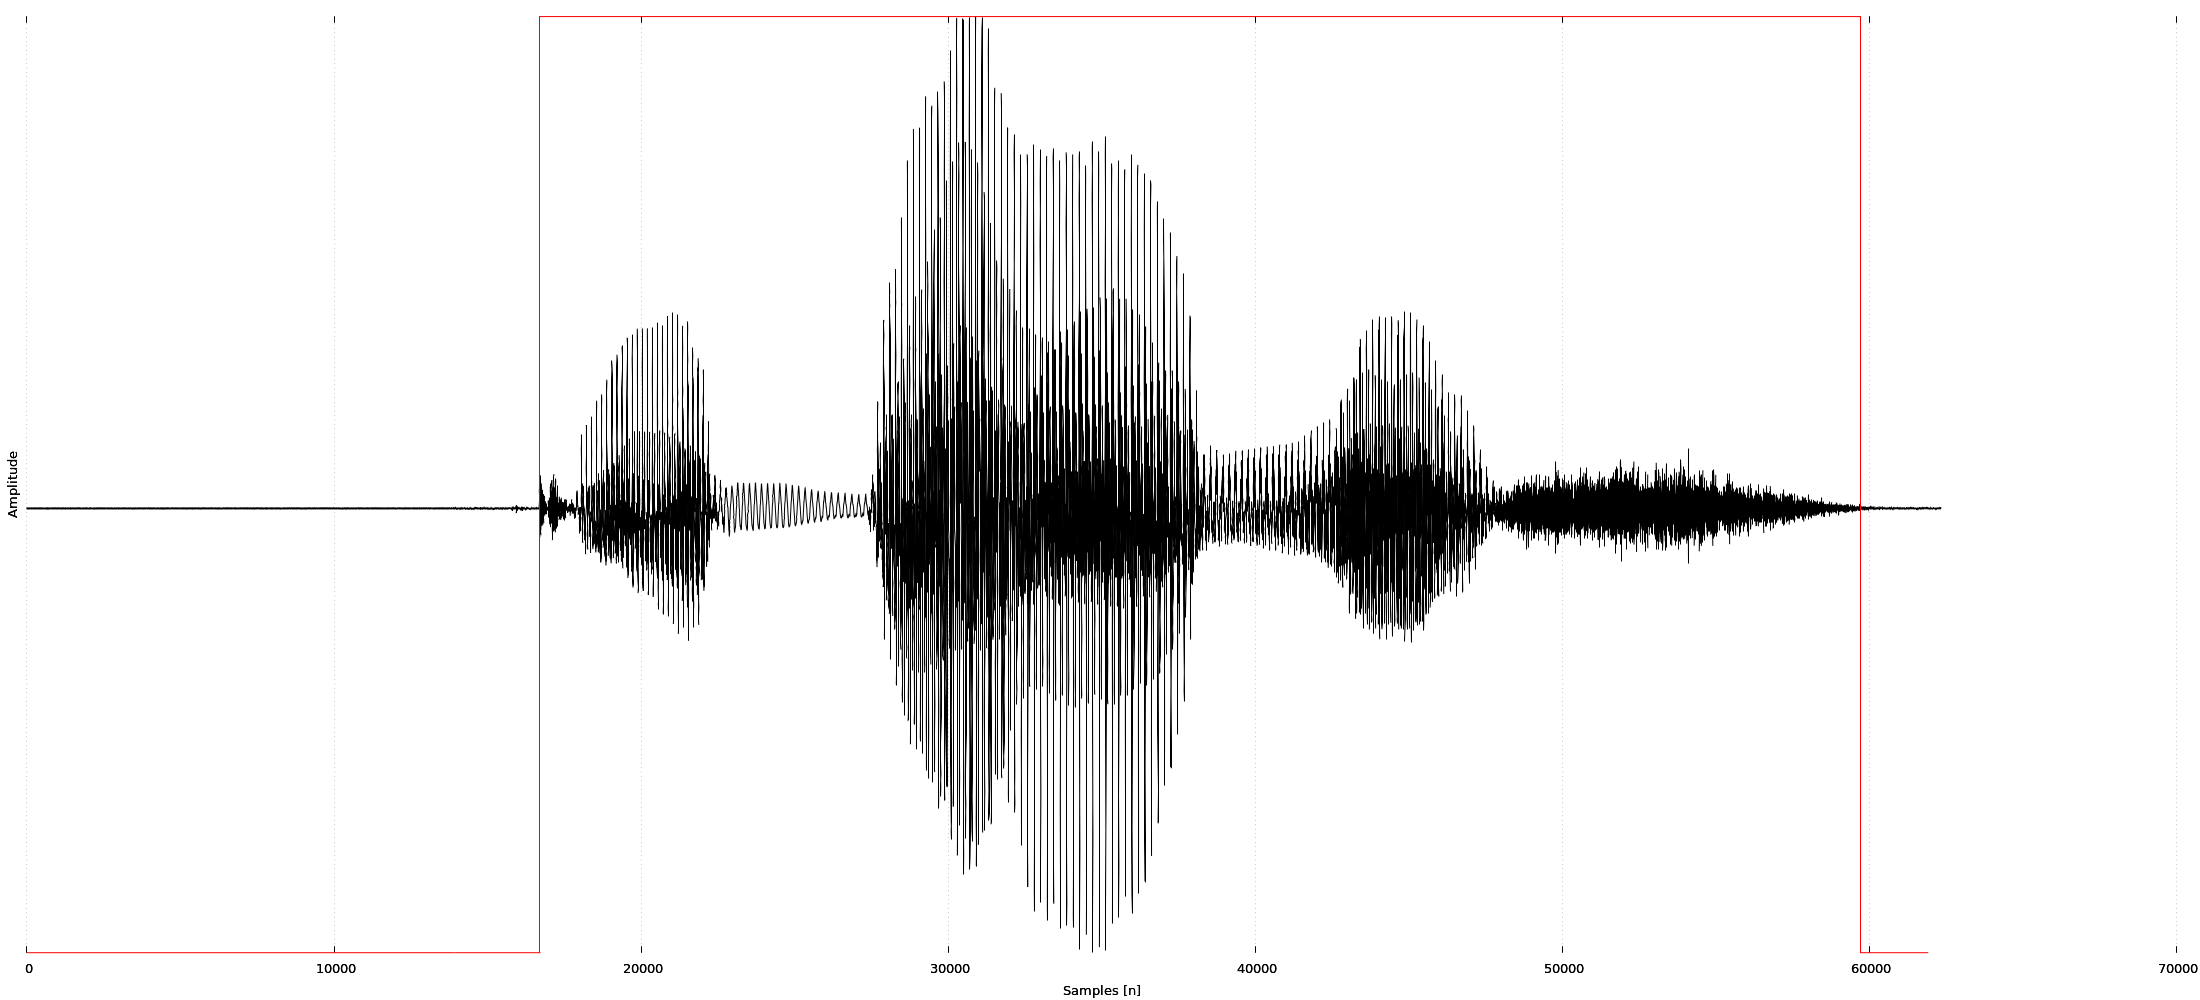
\includegraphics[scale=0.2]{kabanos.png}
			 	\caption{Przebieg czasowy słowa \emph{kabanos} i jego wzorcowa detekcja}\vspace{5mm}
		 \end{center}
	\end{figure}
	
	\begin{figure}
		\begin{center}
			 	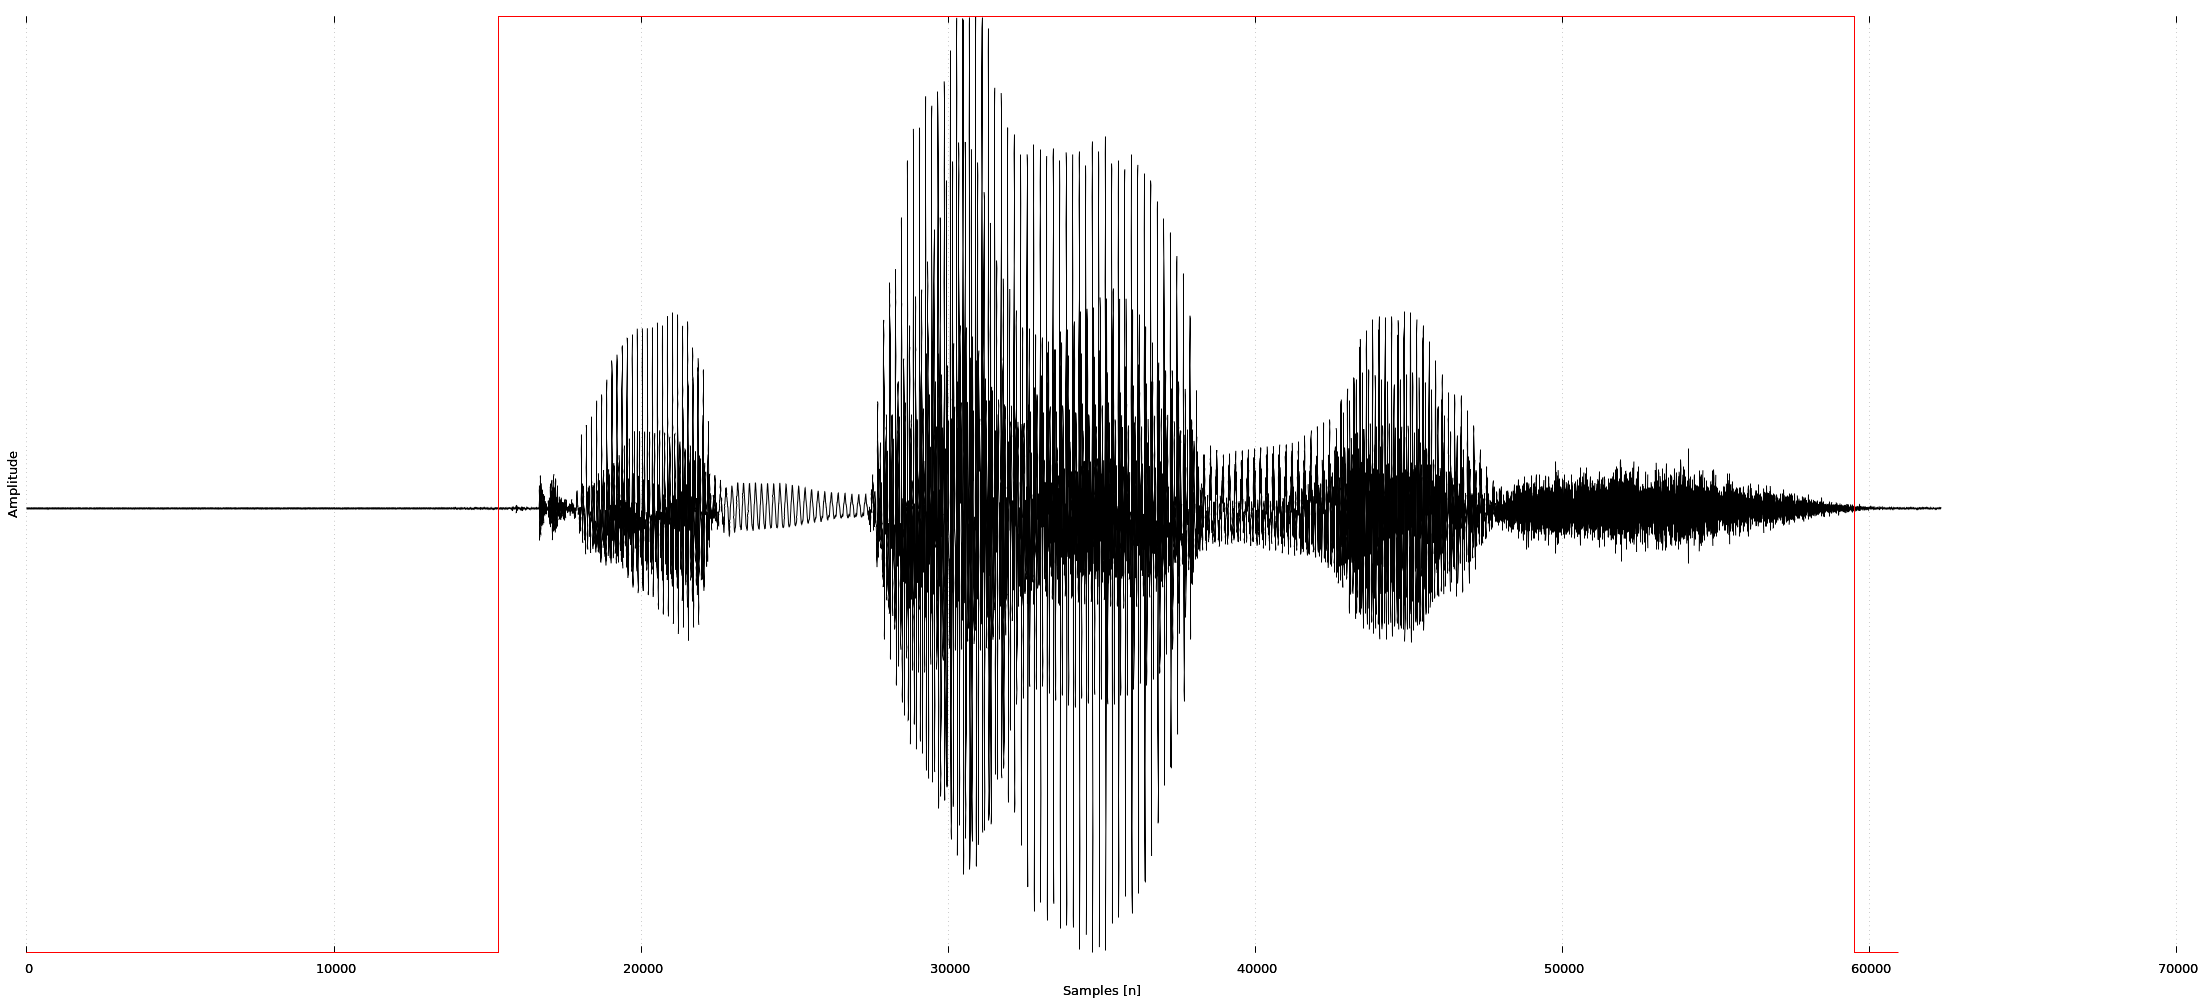
\includegraphics[scale=0.2]{kabanosEnergy.png}
			 	\caption{Wynik detekcji algorytmu bazującego na energii sygnału}\vspace{5mm}
			 	
			 	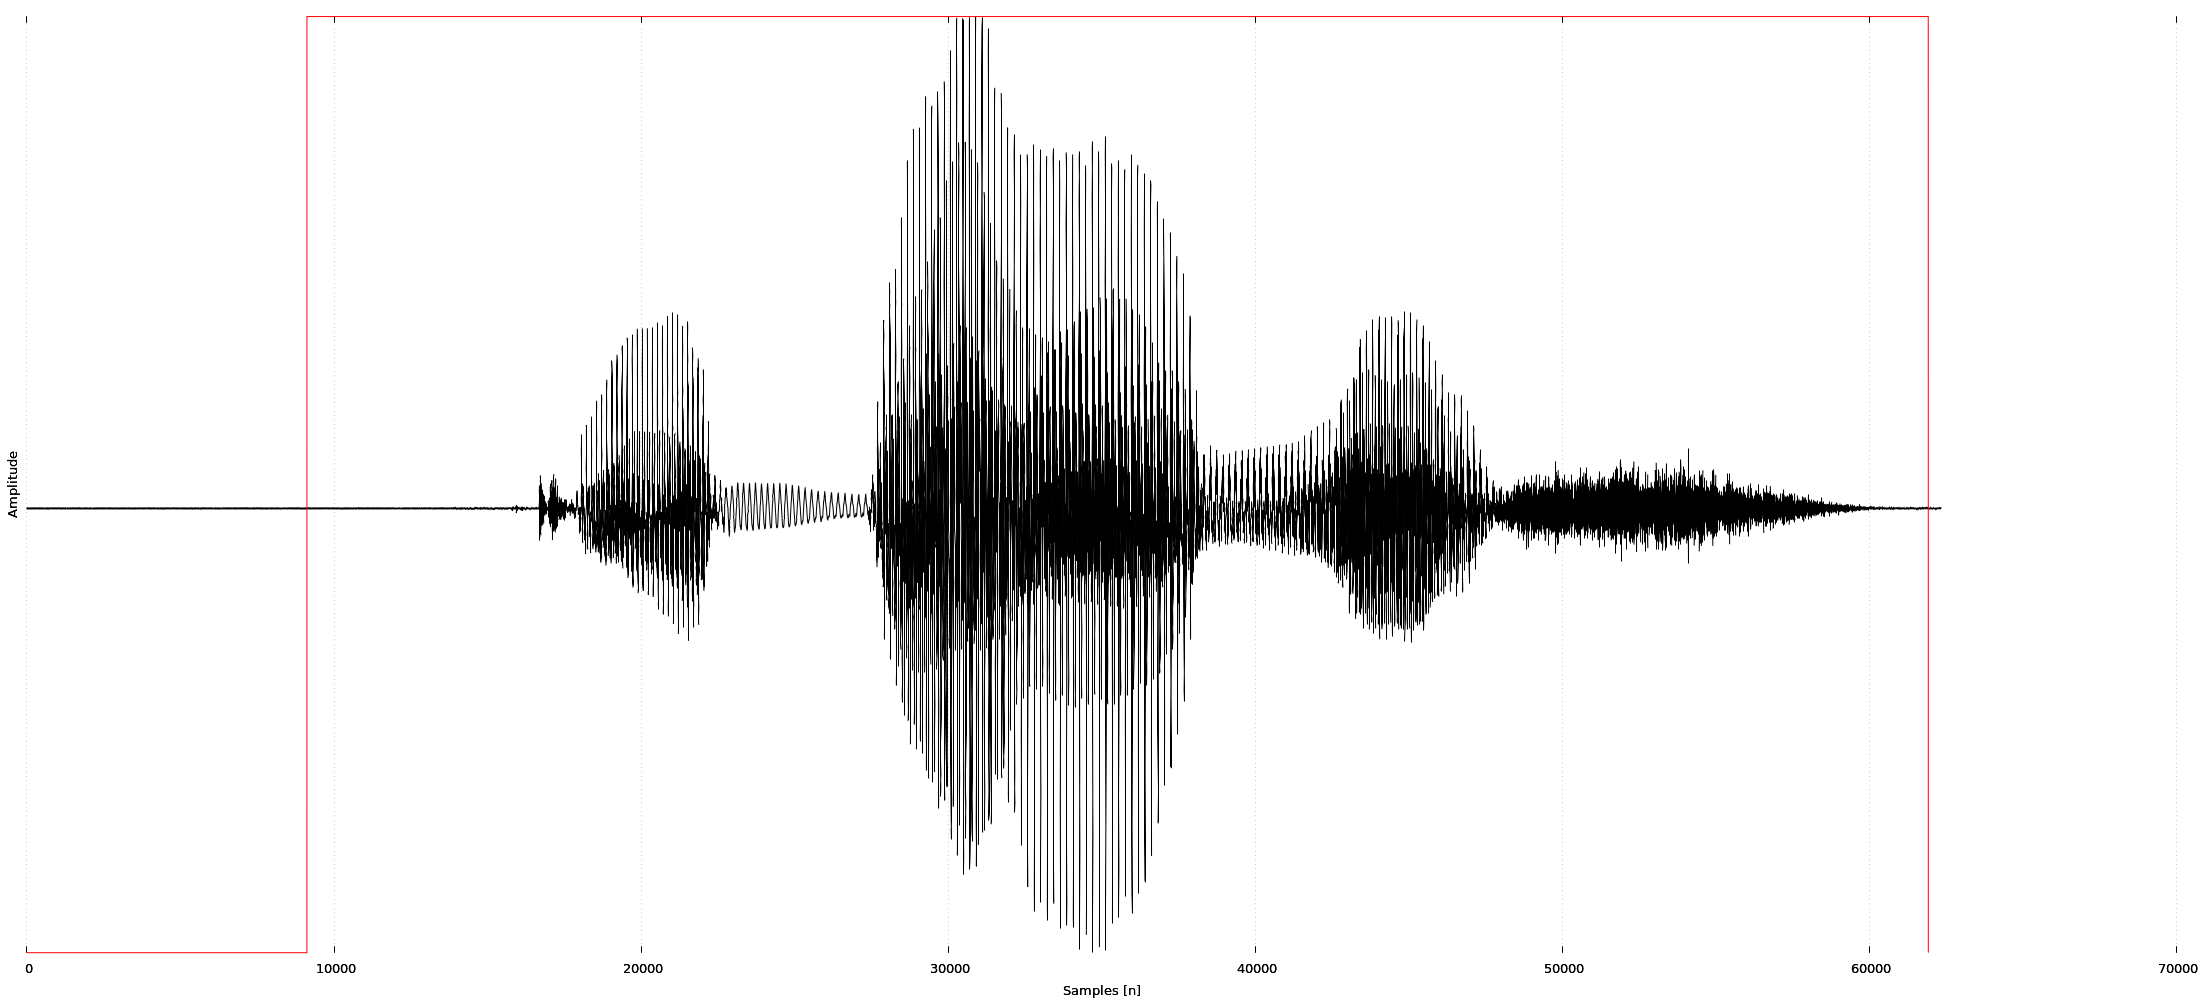
\includegraphics[scale=0.2]{kabanosSFFArticle.png}
			 	\caption{Wynik detekcji algorytmu SFF}\vspace{5mm}
			 	
			 	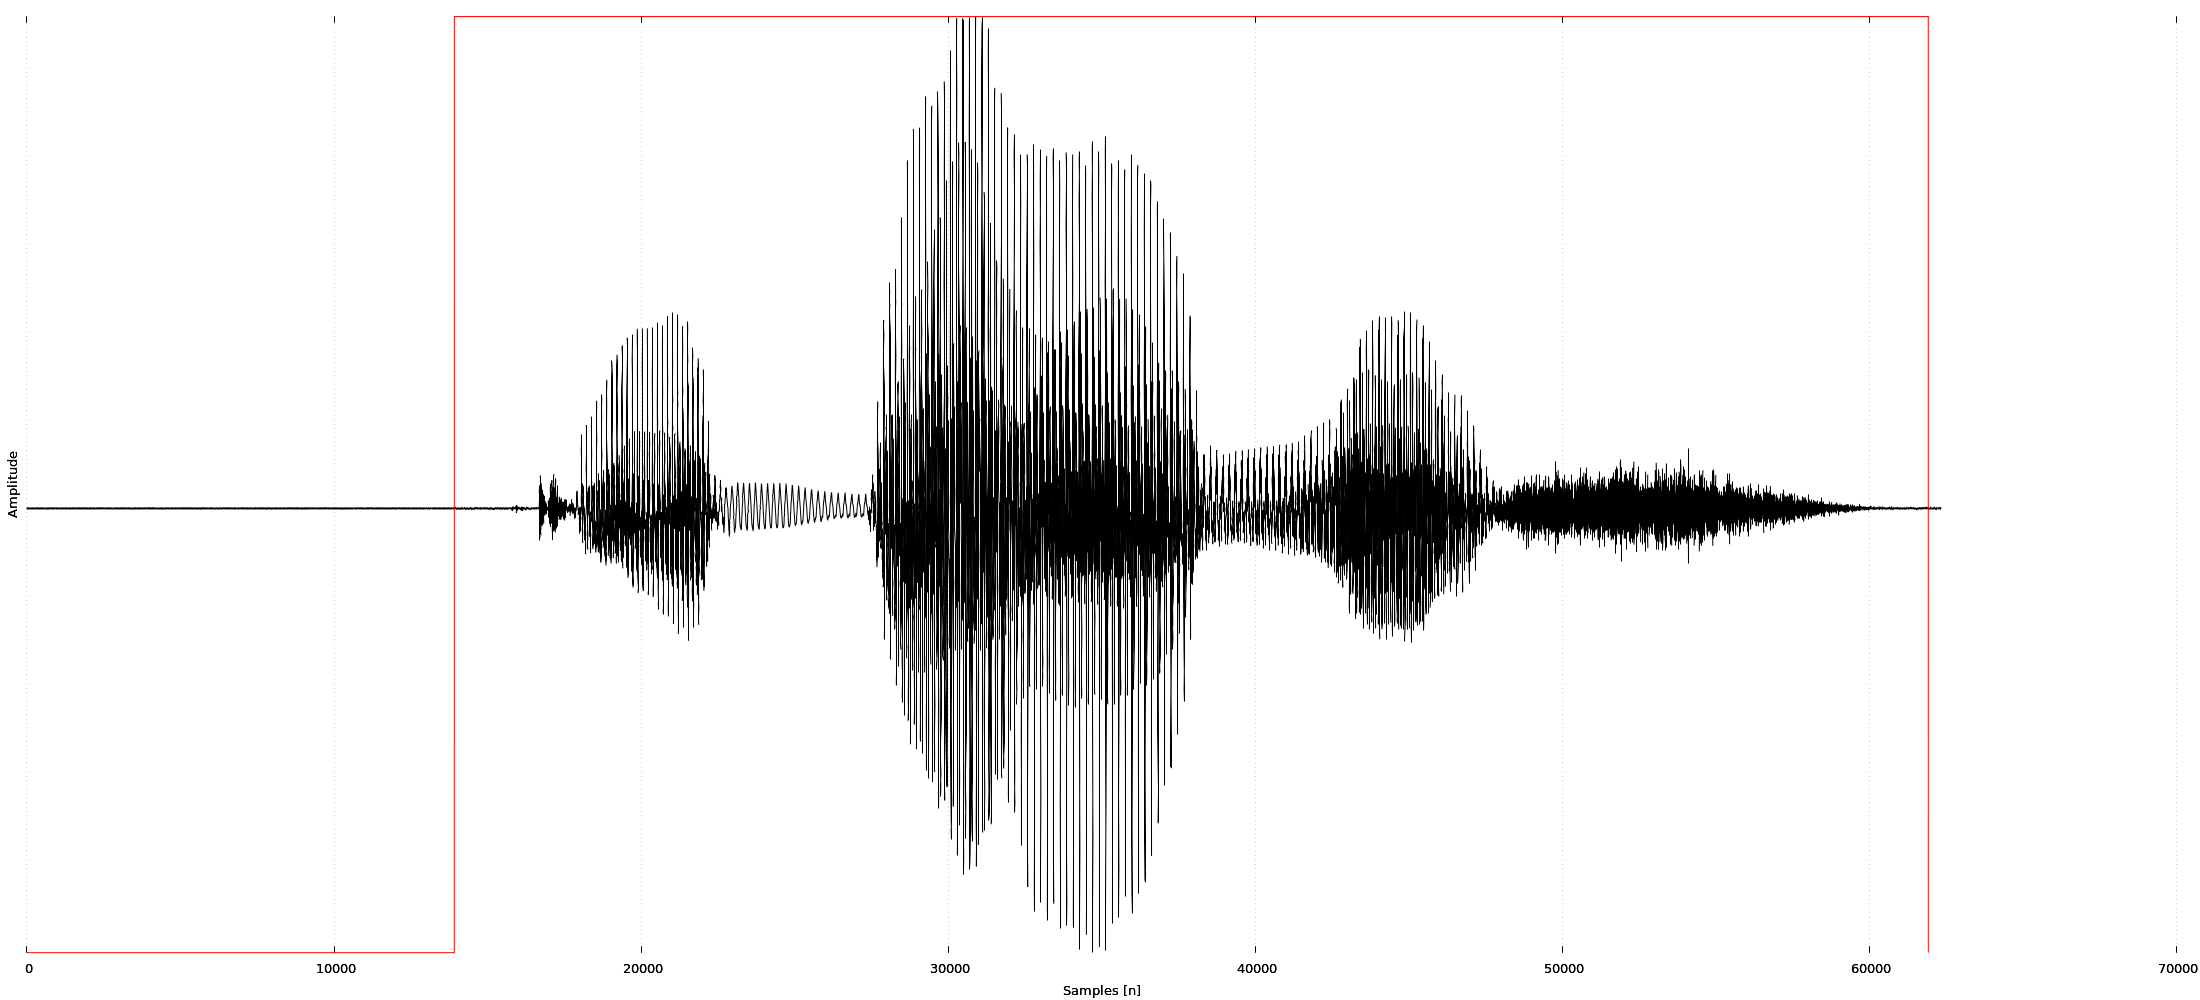
\includegraphics[scale=0.2]{kabanosSFFChanged.png}
			 	\caption{Wynik detekcji algorytmu SFF2}\vspace{5mm}
		\end{center}
	\end{figure}
	
	
	\begin{figure}
		Poniższa tabela przedstawia różnicę w próbkach dla każdego algorytmu, w porównaniu z tymi ustawionymi ręcznie. Przedstawione wartości zostały obliczone zgodnie ze wzorem $| x_{man}-x_{alg} |$, gdzie $x_{man}$ to nr próbki wybranej manualnie, a $x_{alg}$, to numer próbki wybranej przez algorytm. 
	 	\begin{center}
	 		\begin{tabular}{||c c c c c||} 
	 			\hline
			 			 &Wzorzec[nr próbki]& En[nr próbki] & SFF[nr próbki] & SFF2[nr próbki] \\ [0.5ex] 
	 			\hline
	 			Początek & 16705 & 15360 & 9121 & 13921 \\ 
	 			\hline
	 			Koniec & 59712 & 60000 & 61920 & 61920 \\
	 			\hline
	 			SUMA RÓŻNIC  & 0 & 1535 & 9792 & 4992 \\
	 			\hline
	 		\end{tabular}
	 		\caption{Odległość od wzorcowych próbek dla poszczegolnych algorytmów, wyrażona w próbkach}\vspace{5mm}
	 	\end{center}
	 	
	 	\begin{center}
	 		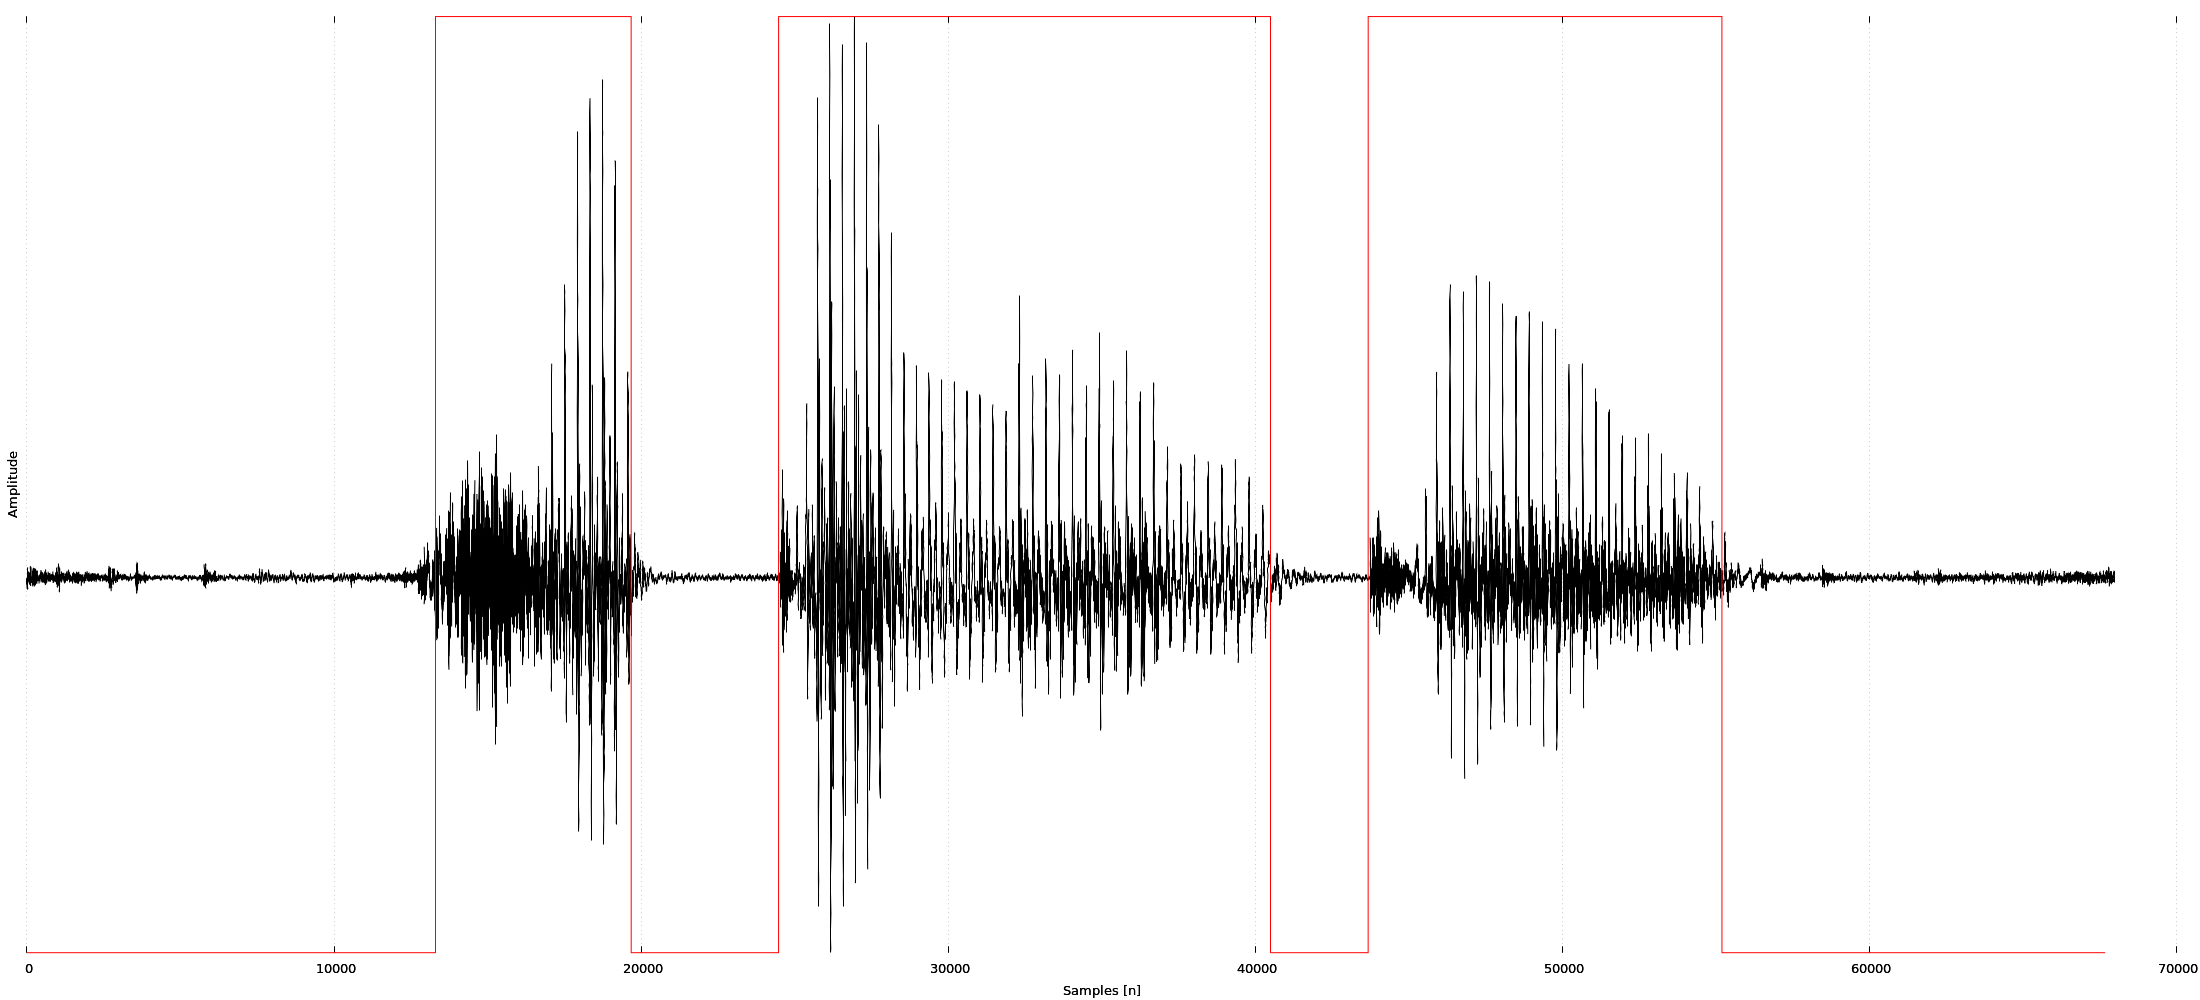
\includegraphics[scale=0.2]{zapamietaj.png}
	 		\caption{Przebieg czasowy słowa \emph{zapamiętaj} i jego wzorcowa detekcja}\vspace{5mm}
	 	\end{center}
	\end{figure}
 
	 
	 \begin{figure}
	 	\begin{center}
	 		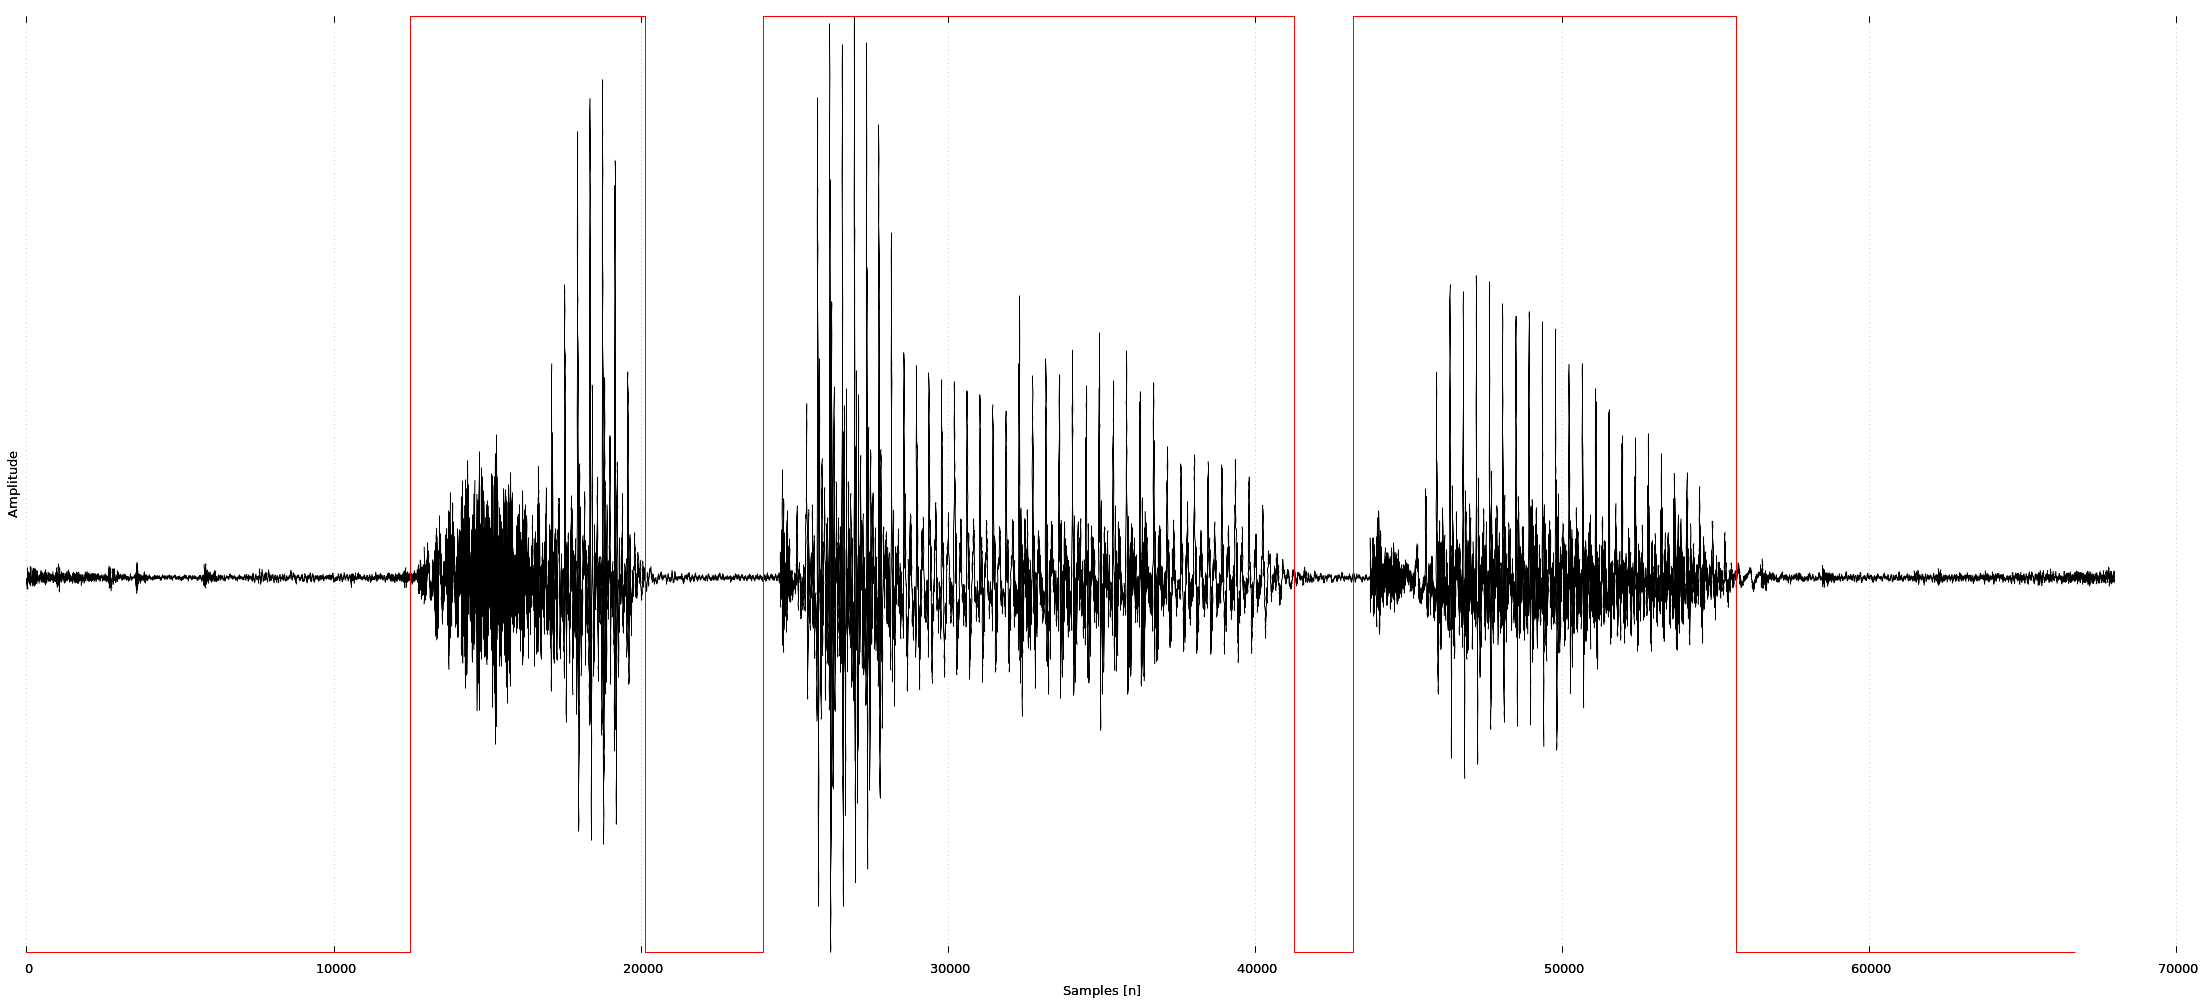
\includegraphics[scale=0.2]{zapamietajEnergy.png}
	 		\caption{Wynik detekcji algorytmu bazującego na energii sygnału}\vspace{5mm}
	 		
	 		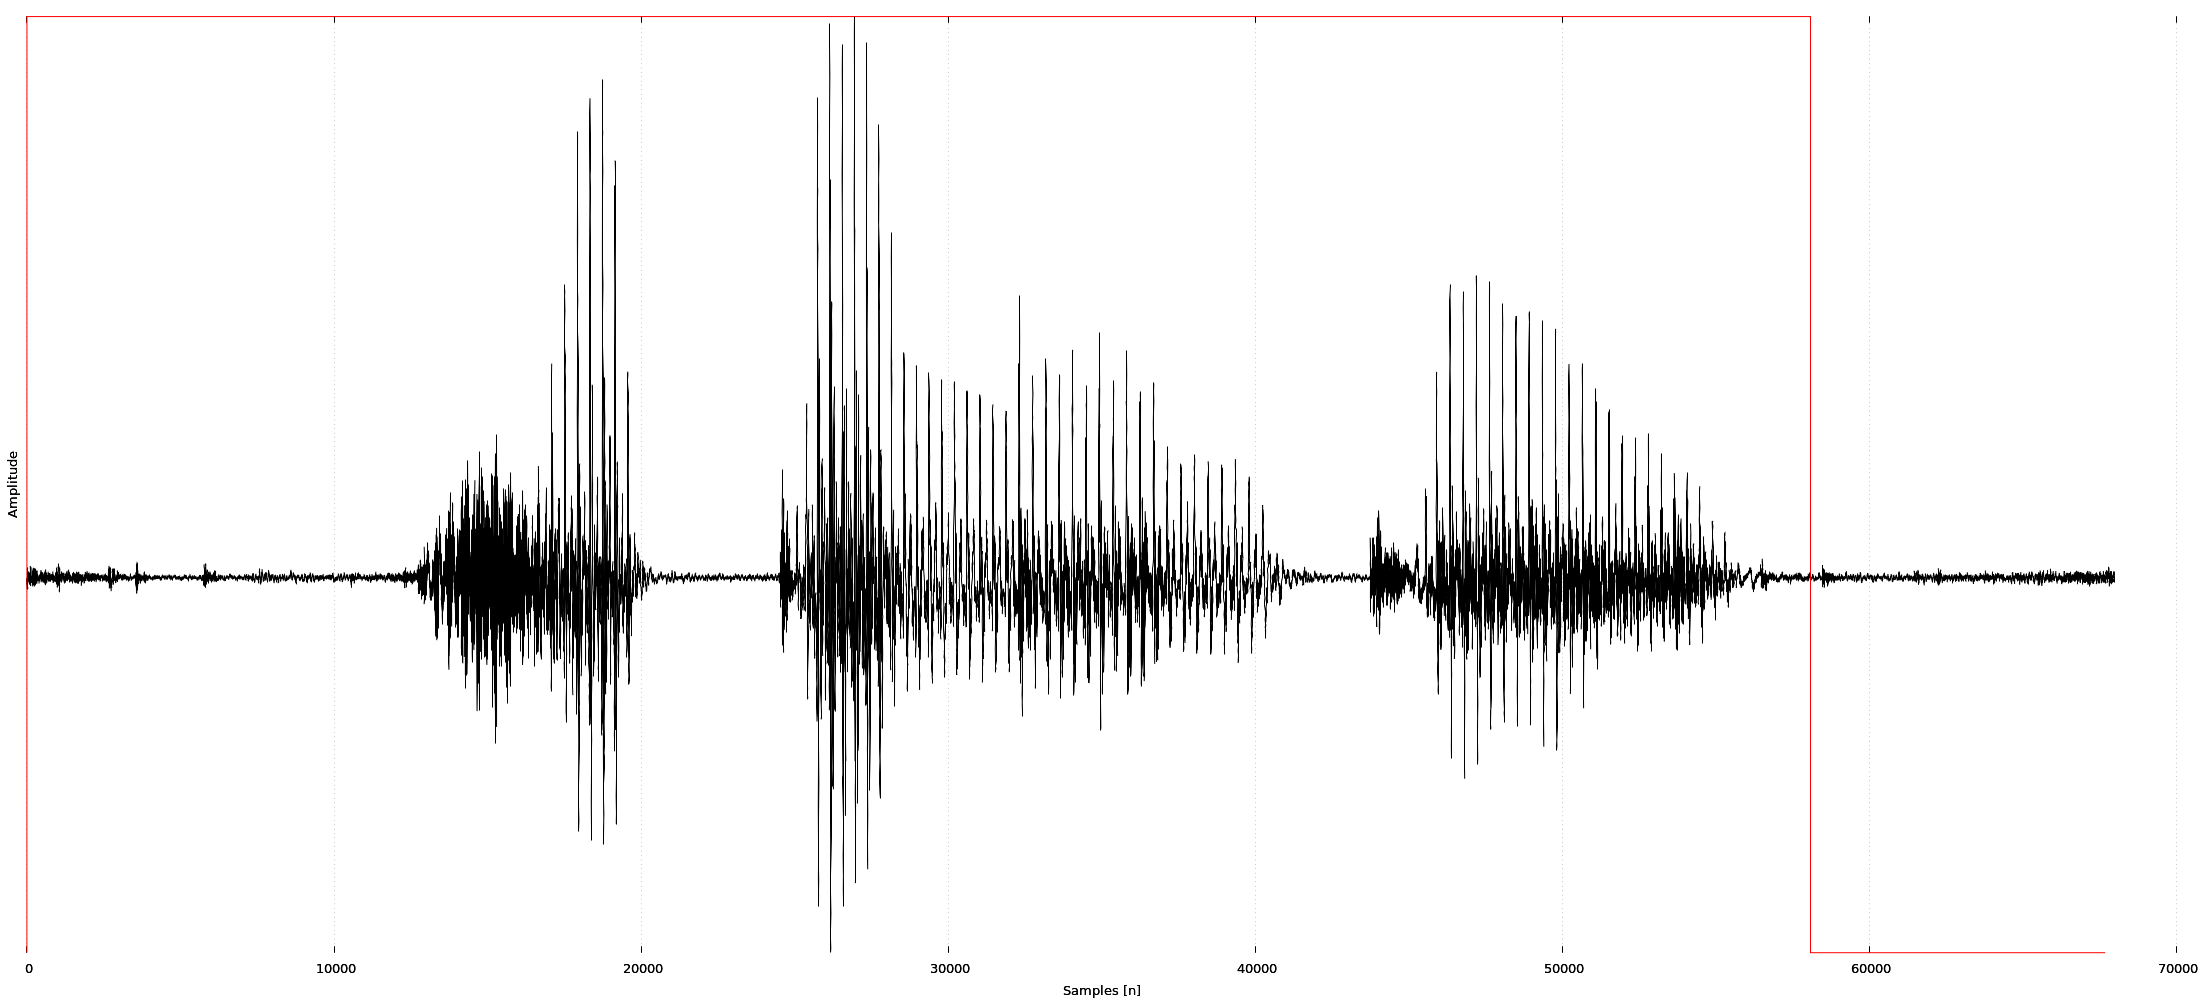
\includegraphics[scale=0.2]{zapamietajSFFArticle.png}
	 		\caption{Wynik detekcji algorytmu SFF}\vspace{5mm}
	 		
	 		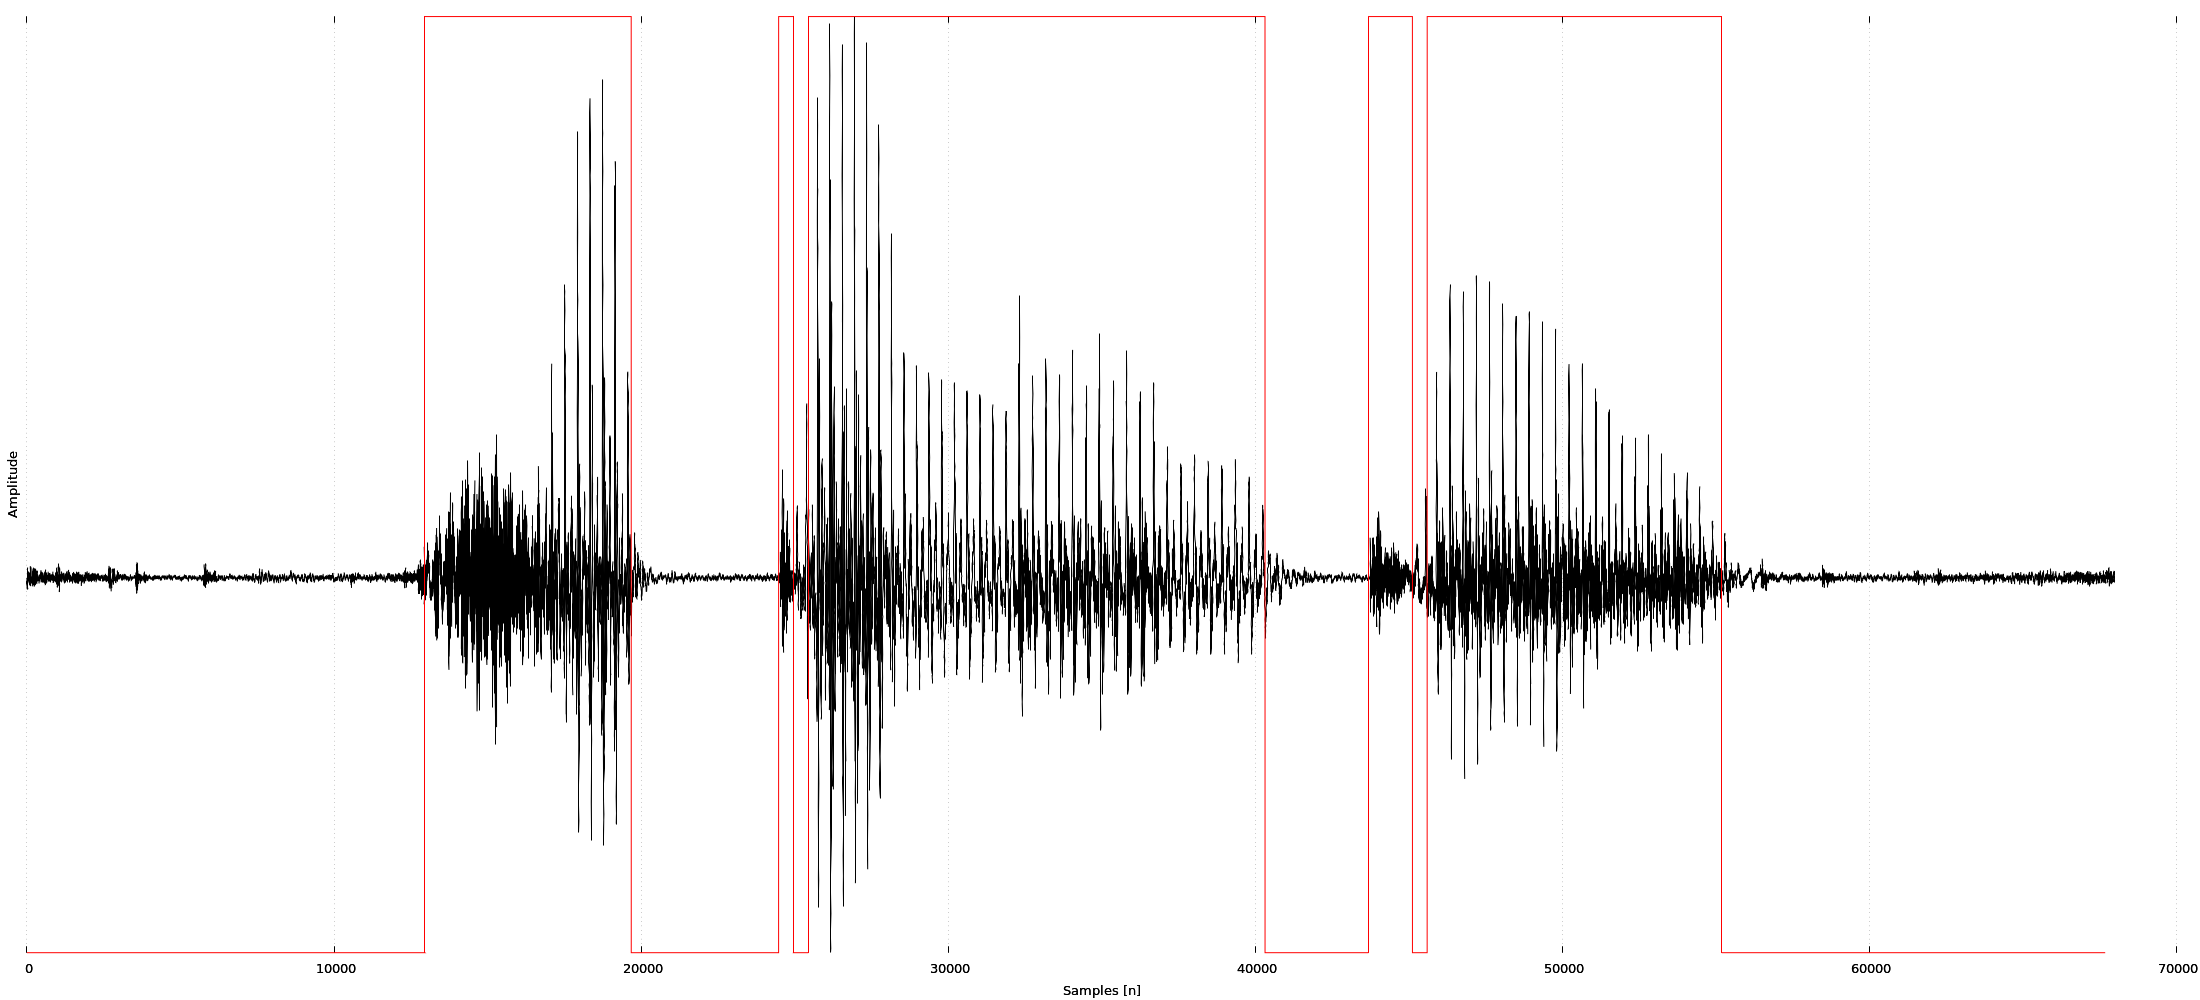
\includegraphics[scale=0.2]{zapamietajSFFChanged.png}
	 		\caption{Wynik detekcji algorytmu SFF2}\vspace{5mm}
	 	\end{center}
	 \end{figure}
	 
	 \begin{figure}
	 	\begin{center}
	 		\begin{tabular}{||c c c c c||} 
	 			\hline
	 			&Wzorzec[nr próbki] & En[nr próbki] & SFF[nr próbki] & SFF2[nr próbki] \\ [0.5ex] 
	 			\hline
	 			Początek1 & 13296 & 12480 & 2 & 12961 \\ 
	 			\hline
	 			Koniec1 & 19680 & 20160 & - & 19681 \\ 
	 			\hline
	 			Początek2 & 24480 & 24000 & - & 24481 \\ 
	 			\hline
	 			Koniec2 & 40512 & 41280 & - & 40321 \\
	 			\hline
	 			Początek3 & 43680 & 43200 & - & 43681\\
	 			\hline
	 			Koniec3 & 55200 & 55680 & 58081 & 55201\\
	 			\hline
	 			SUMA RÓŻNIC & 0 & 3504 & 144527 & 530\\
	 			\hline
	 		\end{tabular}
	 		\caption{Różnice między wzorcowymi próbkami}
	 	\end{center}
	 	
	 	Algorytm SFF2 zdetekował dwa dodatkowe obszary - jeden zawarty między Początek2 i Koniec2, drugi między Początek3 i Koniec3:
	 	\begin{center}
	 		\begin{tabular}{||c c||} 
	 			\hline
	 			&SFF2 \\ [0.5ex] 
	 			\hline
	 			Początek2.1 & 24961 \\ 
	 			\hline
	 			Koniec2.1 & 25441 \\ 
	 			\hline
	 			Początek2.1 & 45121\\ 
	 			\hline
	 			Koniec2.2 &45601\\
	 			\hline
	 		\end{tabular}
	 	\end{center}
	 \end{figure}
	 
	 
 
\begin{figure}

	\section{Wyniki dla ciągów słów}
	Na rysunku 5.9 przedstawiono przebieg czasowy kolejnych słów: \emph{grzech, poprzedni, zapamiętaj, widzenie, ...}, głos damski, a na rysunku 5.13 przebieg czasowy kolejnych  \emph{zapamiętaj}, głos męski, które zostaną poddane detekcji przez algorytmy, które zostały zaprezentowane w poprzednich rozdziałach. Na rysunkach 5.9 oraz 5.13 detekcja została ustawiona manualnie, jako punkt odniesienia dla innych algorytmów.
	Kolejne rysunki zawierają wyniki detekcji.
	\begin{center}
		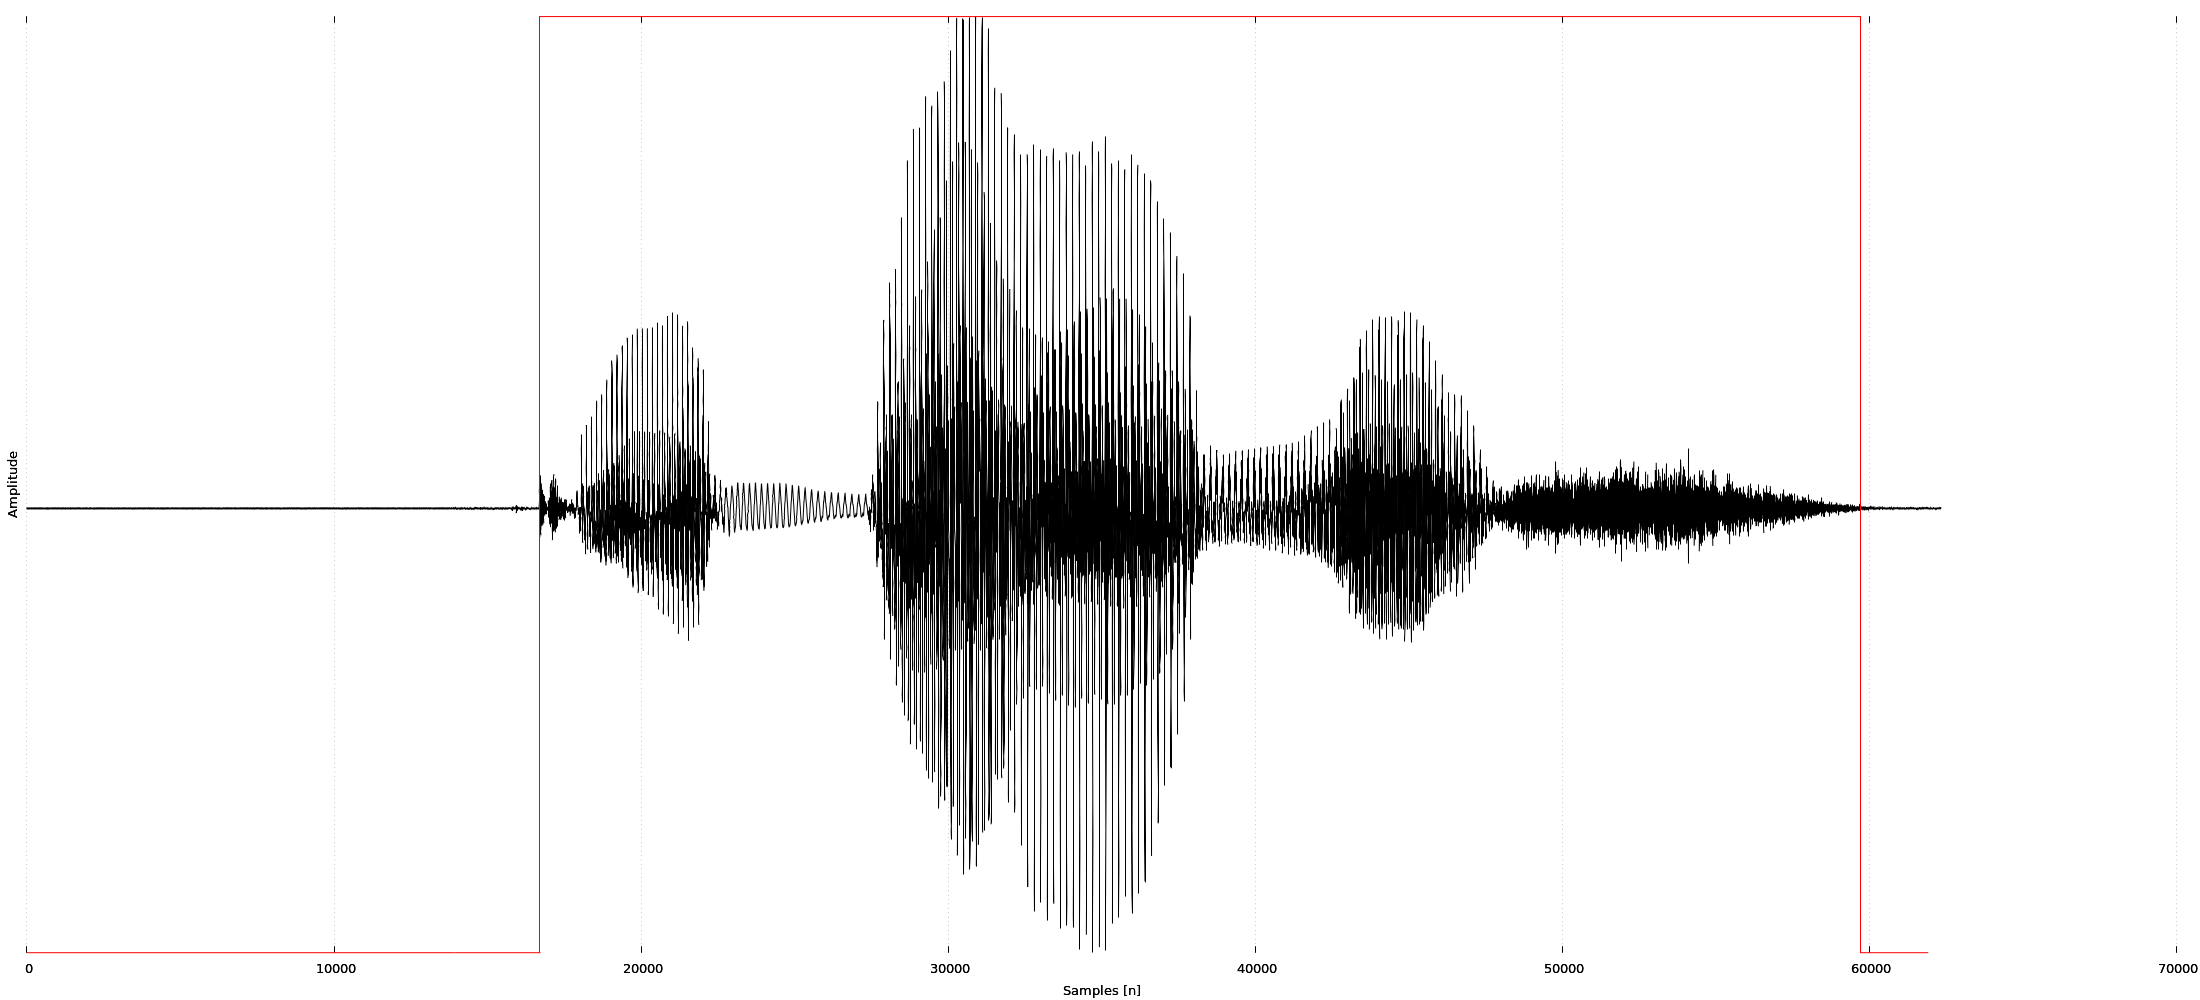
\includegraphics[scale=0.2]{kabanos.png}
		\caption{Przebieg czasowy słowa \emph{kabanos} i jego wzorcowa detekcja}\vspace{5mm}
	\end{center}
\end{figure}

\begin{figure}
	\begin{center}
		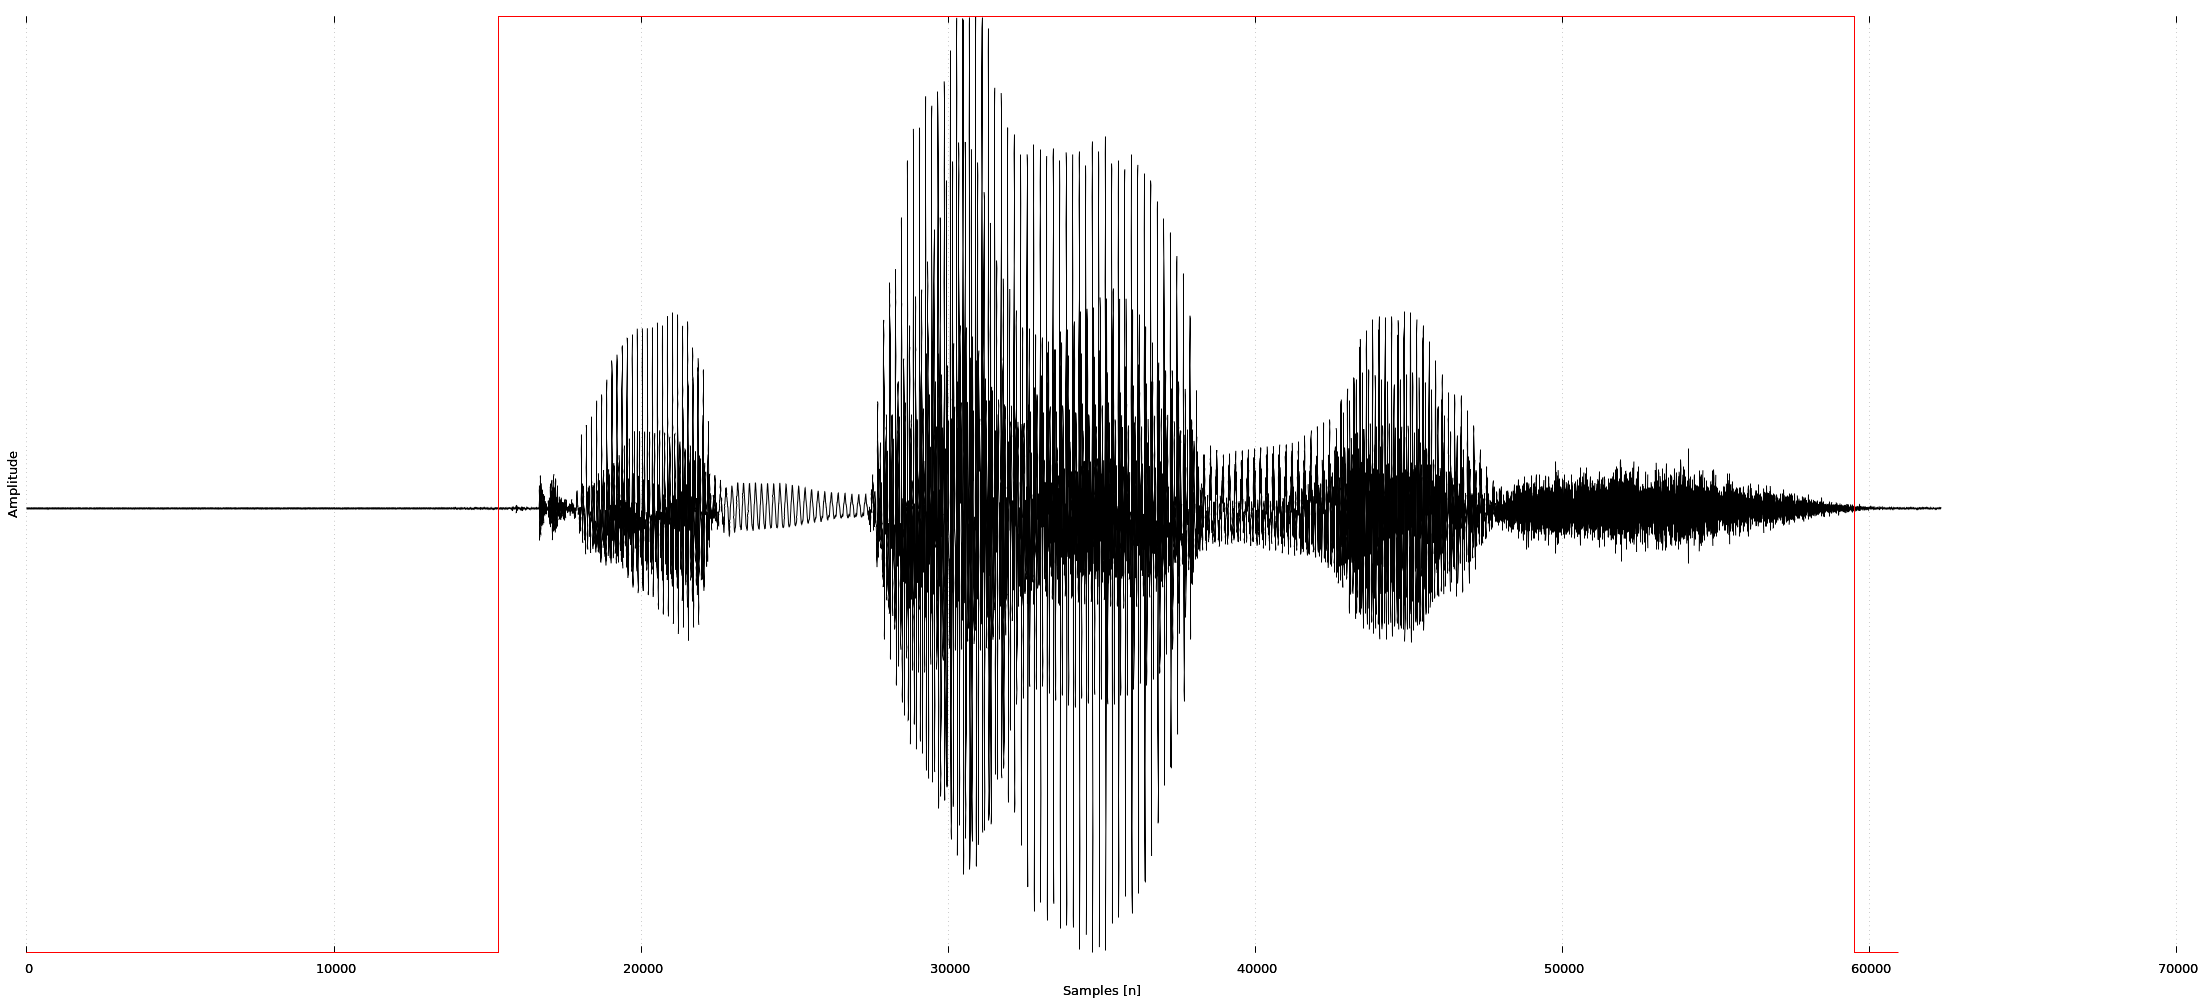
\includegraphics[scale=0.2]{kabanosEnergy.png}
		\caption{Wynik detekcji algorytmu bazującego na energii sygnału}\vspace{5mm}
		
		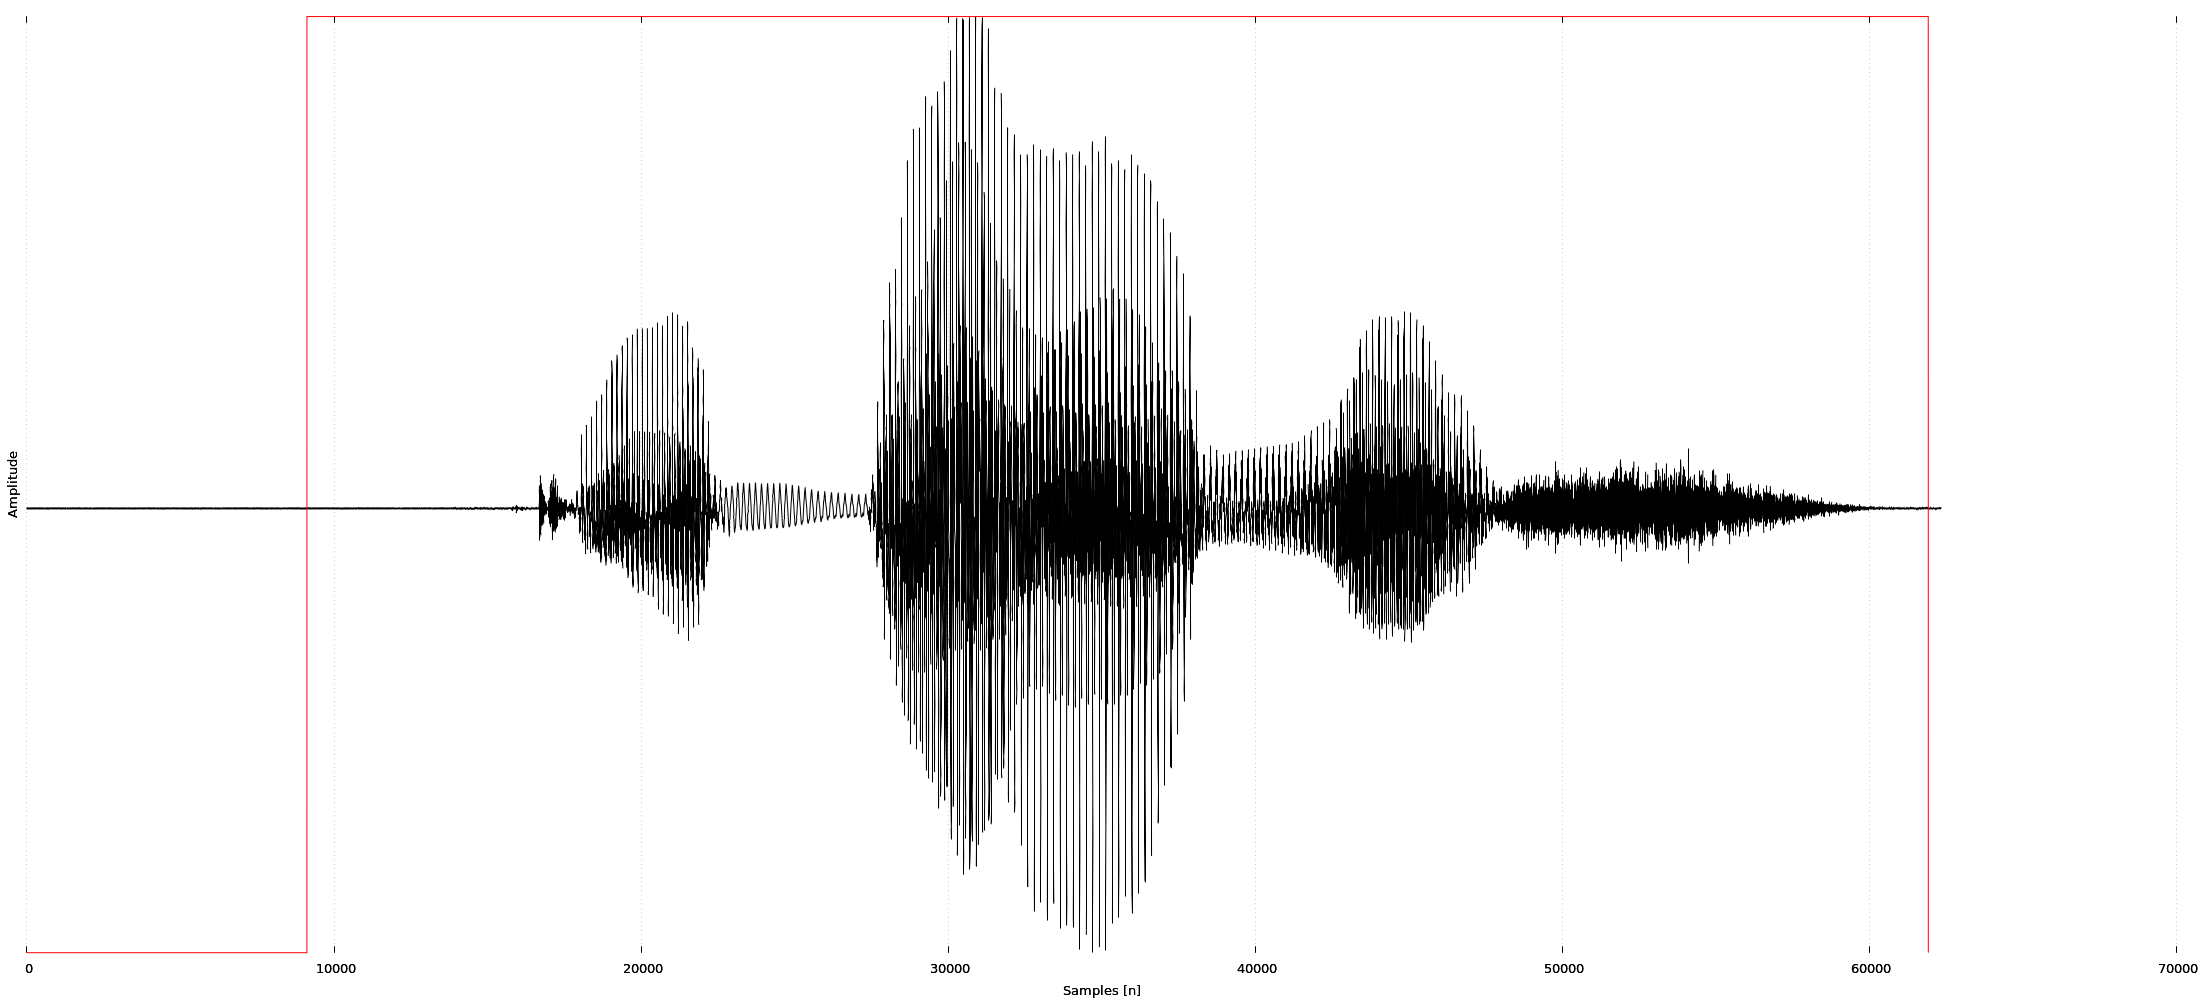
\includegraphics[scale=0.2]{kabanosSFFArticle.png}
		\caption{Wynik detekcji algorytmu SFF}\vspace{5mm}
		
		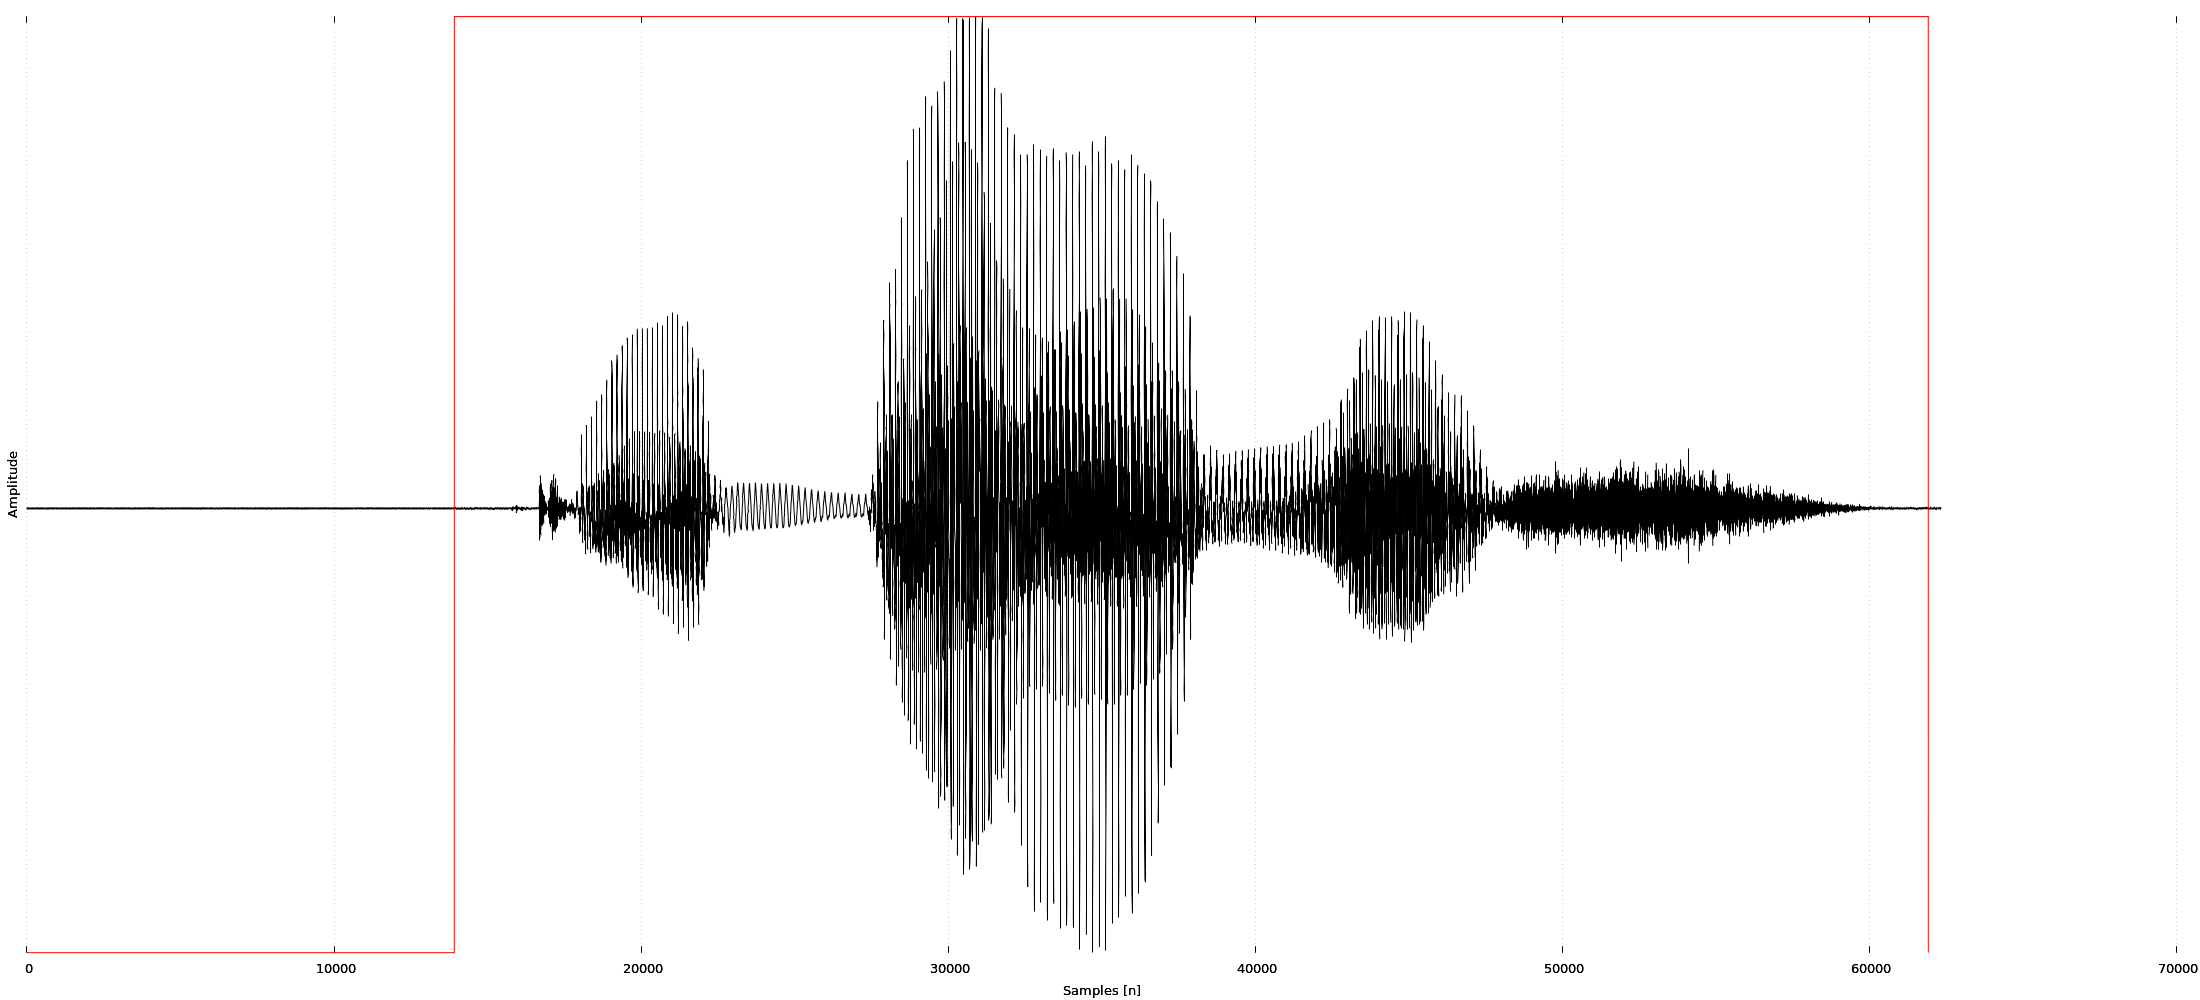
\includegraphics[scale=0.2]{kabanosSFFChanged.png}
		\caption{Wynik detekcji algorytmu SFF2}\vspace{5mm}
	\end{center}
\end{figure}


\begin{figure}
	Poniższa tabela przedstawia różnicę w próbkach dla każdego algorytmu, w porównaniu z tymi ustawionymi ręcznie. Przedstawione wartości zostały obliczone zgodnie ze wzorem $| x_{man}-x_{alg} |$, gdzie $x_{man}$ to nr próbkik wybranej manualnie, a $x_{alg}$, to numer próbki wybranej przez algorytm. 
	\begin{center}
		\begin{tabular}{||c c c c||} 
			\hline
			& En & SFF & SFF2 \\ [0.5ex] 
			\hline\hline
			Początek & 16703 & 7103 & 2783 \\ 
			\hline
			Koniec & 1248 & 2208 & 2208 \\
			\hline
		\end{tabular}
	\end{center}
	
	\begin{center}
		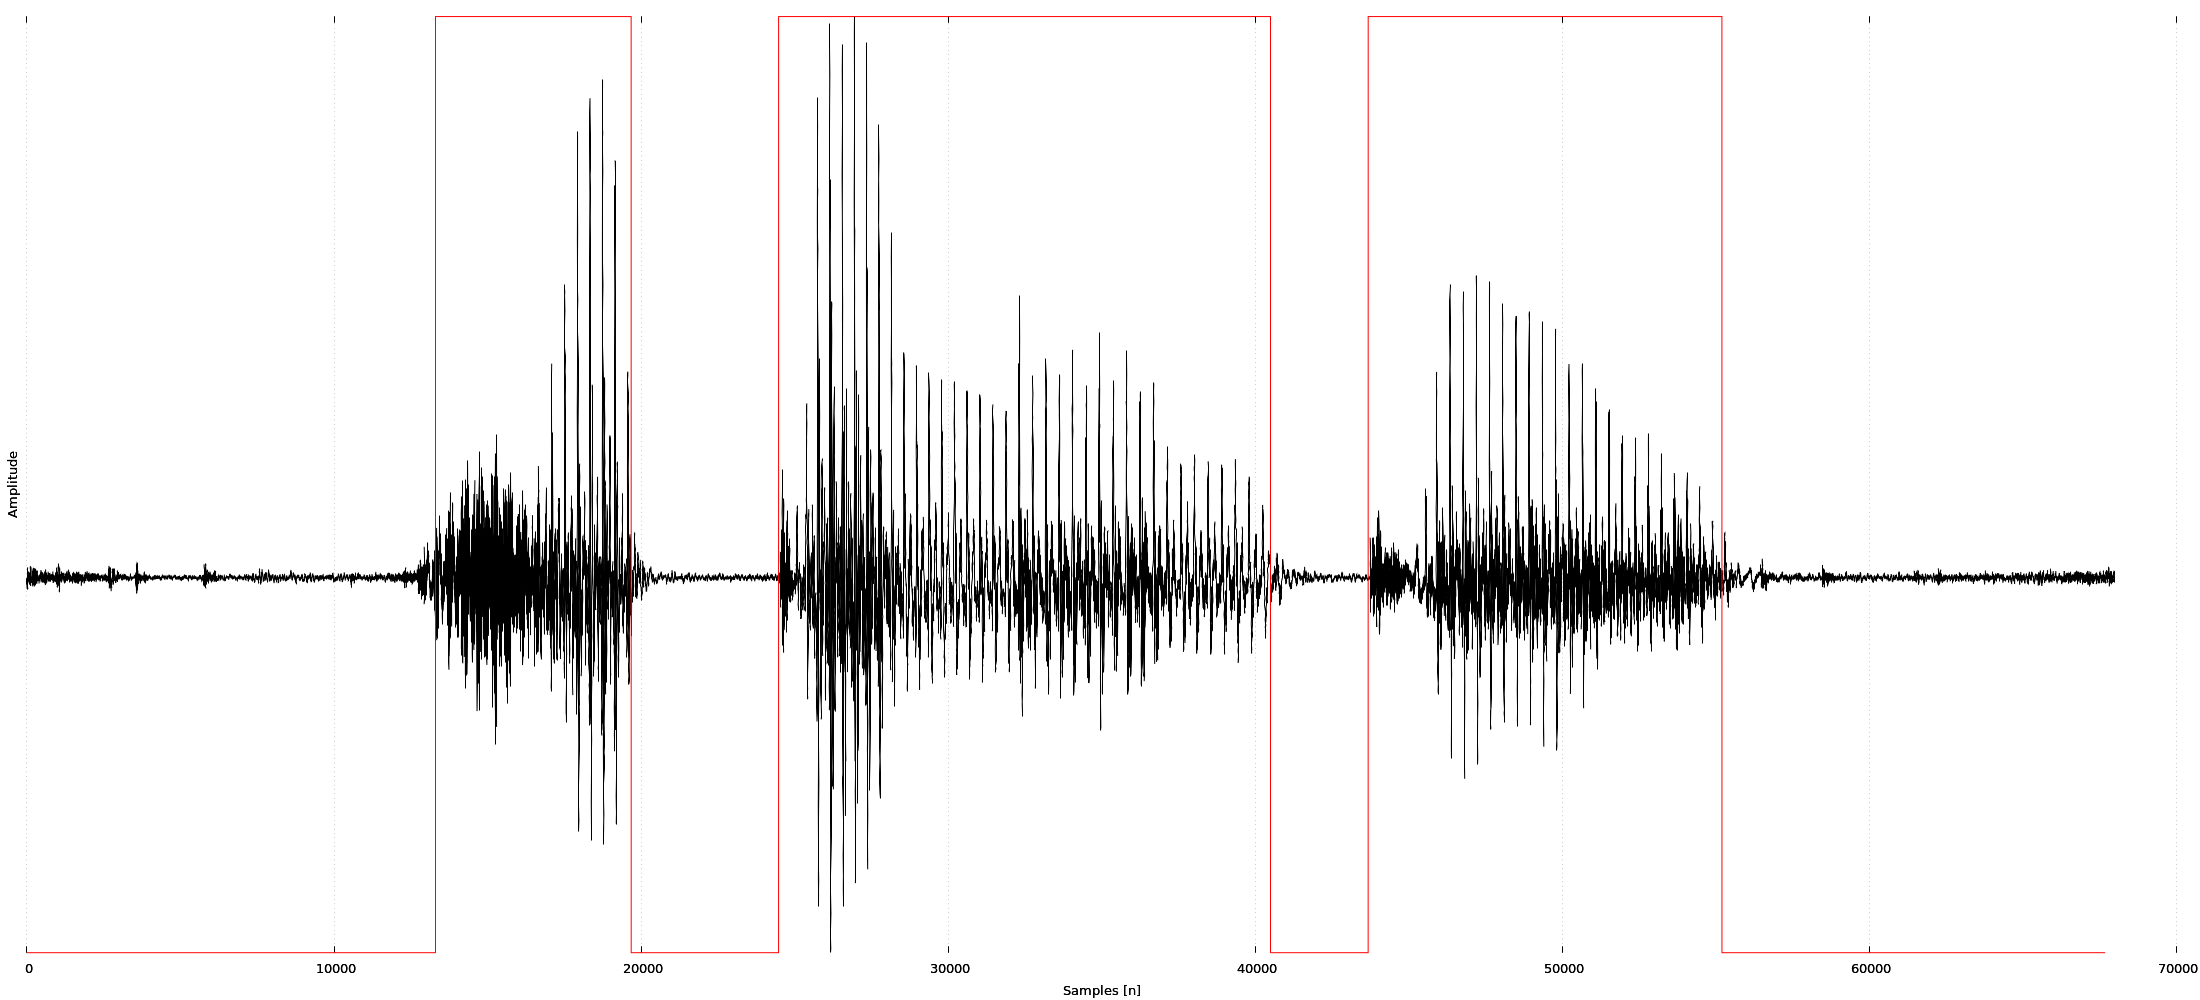
\includegraphics[scale=0.2]{zapamietaj.png}
		\caption{Przebieg czasowy słowa \emph{zapamiętaj} i jego wzorcowa detekcja}\vspace{5mm}
	\end{center}
\end{figure}


\chapter{Podsumowanie}

\addcontentsline{toc}{chapter}{Bibliografia} %utworzenie w spisie treści pozycji Bibliografia
\bibliography{bibliografia} % wstawia bibliografię korzystając z pliku bibliografia.bib - dotyczy BibTeXa, jeżeli nie korzystamy z BibTeXa należy użyć otoczenia thebibliography
%biologiczny proces
%http://otworzksiazke.pl/images/ksiazki/sygnal_mowy/sygnal_mowy.pdf
%
%http://www.iaeng.org/IJCS/issues_v36/issue_4/IJCS_36_4_16.pdf


%opcjonalnie może się tu pojawić spis rysunków i tabel
 \listoffigures
 \listoftables
\end{document}

